\documentclass[conference]{IEEEtran}

% *** PACKAGES ***
\usepackage{amsmath}
\usepackage{graphicx}
\usepackage{grffile}
\usepackage{listings}
\usepackage{xcolor}
\usepackage{float}
\usepackage{booktabs}
\usepackage{tikz}
\usepackage{subcaption}
\usepackage{hyperref}
\usepackage{amssymb}

\begin{document}

\title{VLSI Project \\ 4-Bit Carry Lookahead Adder}

\author{
    \IEEEauthorblockN{Sudhanva Joshi - 2023102022}
    \IEEEauthorblockA{ECE, IIIT Hyderabad, Monsoon 2024 \\
    Instructor: Dr. Abhishek Shrivastava}
}

\maketitle

\begin{abstract}
    This report details the design of a 4-bit Carry Lookahead Adder, 
    emphasizing its high-speed performance through parallel carry computation
    by eliminating sequential carry propagation. The pipeline to test this 
    model has been expounded upon below. \\
    \textbf{Note:} All corresponding files are included in their respective folders.   
\end{abstract}

% \begin{IEEEkeywords}
% \end{IEEEkeywords}

% *** MAIN BODY ***
\section{Adder Structure}
The following CLA Adder, along with D Flip-Flop conditions given, is implemented. Each sum output drives an inverter sized to meet 
project specifications.
\begin{figure}[H] 
    \centering
    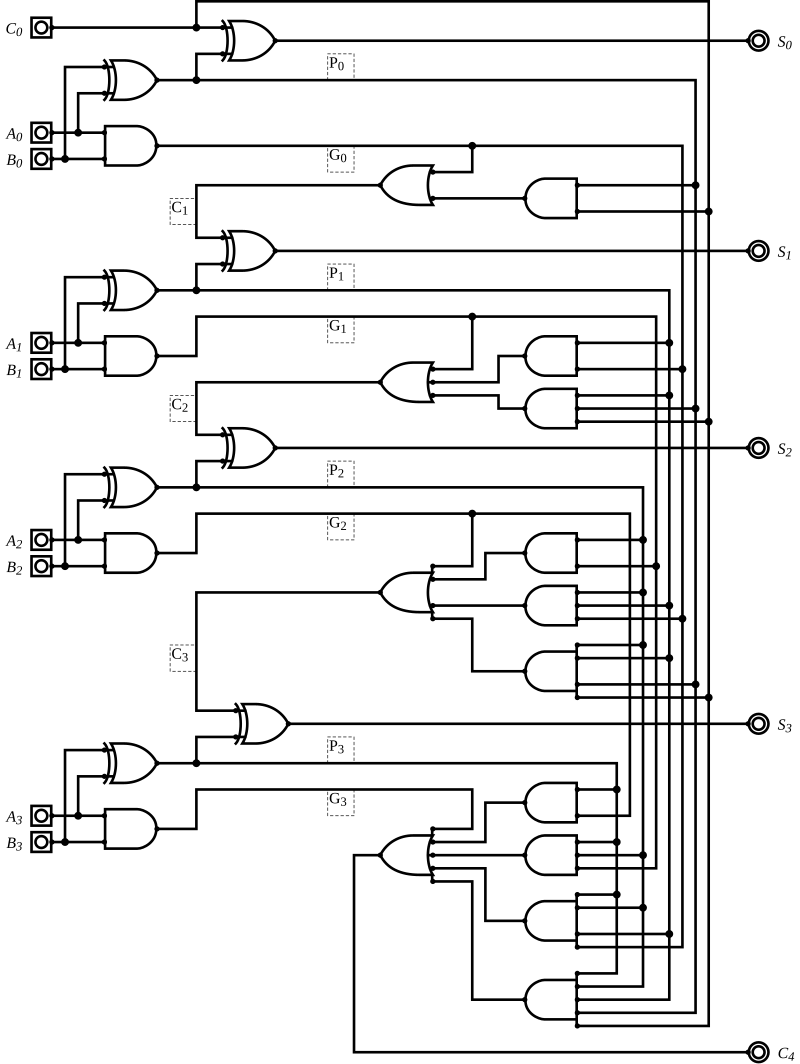
\includegraphics[width=0.2\textwidth]{/home/sudhujoshi/Desktop/Sem_3/VLSI/VLSI_Project/ReportDump/circuit_diagrams/cla_full.png}
    \caption{Circuit Diagram, 4-Bit CLA Adder} 
\end{figure}
The CLA adder accelerates binary addition by precomputing carry signals. It uses the concepts of \textbf{generate} ($G_i$) and \textbf{propagate} ($P_i$) signals defined for each bit as:

\[
G_i = A_i \cdot B_i, \quad P_i = A_i + B_i
\]

where $A_i$ and $B_i$ are the input bits. The carry signals are calculated recursively as:

\[
C_{i+1} = G_i + (P_i \cdot C_i)
\]

The sum bits are computed as:
\[
S_i = P_i \oplus C_i
\]

This approach eliminates the sequential carry propagation delay, enabling faster computation for large bit-width adders. The CLA uses lookahead logic to compute all carries simultaneously, leveraging the recursive nature of $C_i$.
\section{Design Details}
Given below are design choices of each implementation used along with general justification for the choice of topology used.
\\
Transistor sizing follows \( W_p/W_n = 20\lambda/10\lambda \), where \( \lambda = 0.09\mu m \), 
ensuring balanced performance and area.
\\ 
Static CMOS Logic is used in N-Input OR, AND Gate implementation. i.e.
\\
Count for N-Input OR \& AND Gates = 2*N+2 Transistors.
\\
Sizing Transistors to keep Rise \& Fall Times even while being able to drive given load, 
we have the following relation to account for load.

\[
\frac{W_{p}}{W_{n}} = 2
\]
\[
W_{p} = 2\cdot W_{inv}
\]
\[
W_{n} = 1\cdot W_{inv}
\]



\subsection{XOR Logic}
\textbf{Transmission Gate} is used here for the reasons below.
\begin{itemize}
\item \textbf{Reduced Transistor Count:} Compared to the Static CMOS Logic using 8 Transistors, 6 Transistors are used.
\item \textbf{Output Voltage Levels:} The PTL Implementation for XOR using MUX Logic yields poor Output Voltage Levels, which isn't a problem for the topology used here.
\item \textbf{Delay, Power Benefits:} Due to better sizing and performance, power and delay offered by this design is more favourable.
\end{itemize}

\begin{figure}[H] 
    \centering
    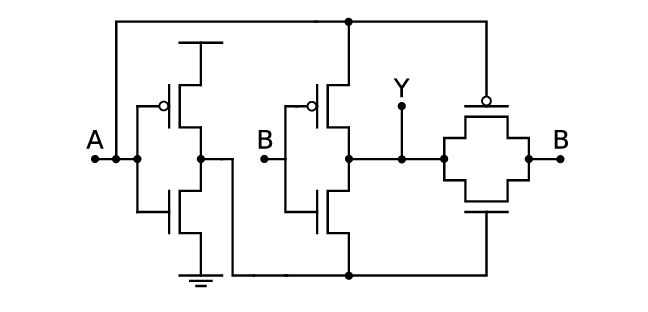
\includegraphics[width=0.5\textwidth]{/home/sudhujoshi/Desktop/Sem_3/VLSI/VLSI_Project/ReportDump/circuit_diagrams/exor_transmission.png}
    \caption{XOR Circuit Diagram, Transmission Gate} 
\end{figure}

\subsection{D Flip-Flop}
\textbf{True Single Phase Clock (TSPC)} is used here for the following reasons:
\begin{itemize}
    \item \textbf{Reduced Transistor Count:} Compared to the Static CMOS Logic using 18 Transistors, 11 Transistors are used here.
    \item \textbf{Single Clock Advantage:} Single Clock Implementation alleviates concerns of multi-clock synchronization, improving clock skew discrepancies.
\end{itemize}
\begin{figure}[H] 
    \centering
    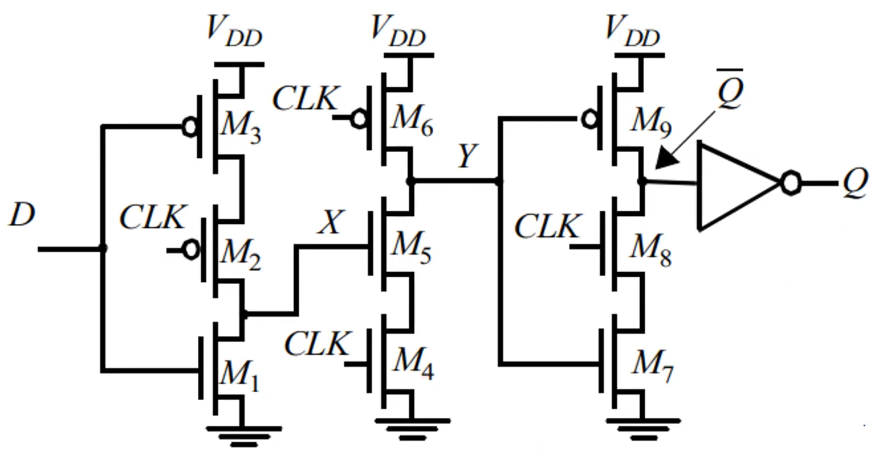
\includegraphics[width=0.4\textwidth]{/home/sudhujoshi/Desktop/Sem_3/VLSI/VLSI_Project/ReportDump/circuit_diagrams/d_ff_tspc.png}
    \caption{Waveform, NGSpice Netlist} 
\end{figure}


\section{Simulation Results}
\subsection{AND Logic}
\subsubsection{AND2}
\begin{figure}[H] 
    \centering
    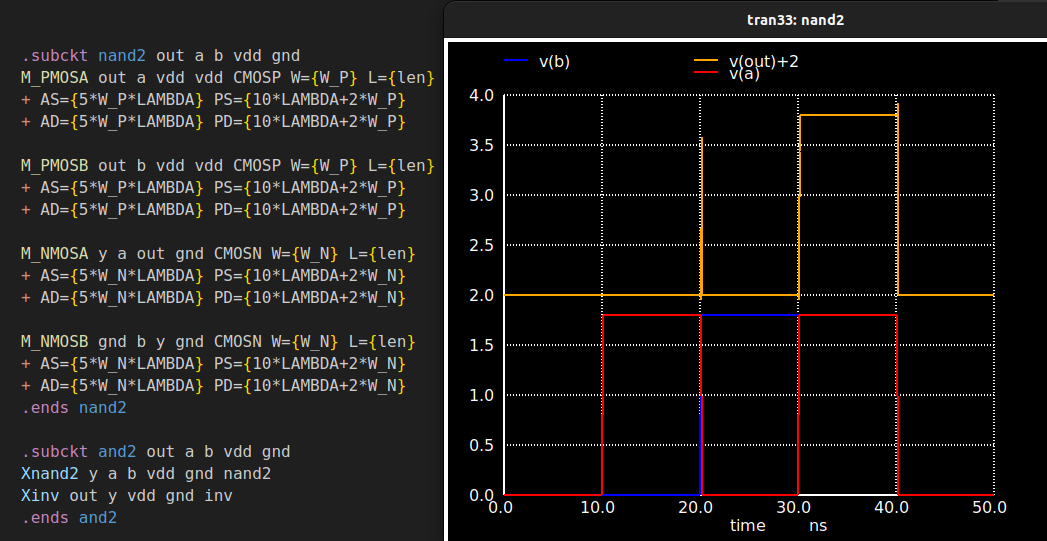
\includegraphics[width=0.4\textwidth]{/home/sudhujoshi/Desktop/Sem_3/VLSI/VLSI_Project/ReportDump/netlist_ss/nand2.png}
    \caption{AND2, Static CMOS Logic} 
\end{figure}
\subsubsection{AND3}
\begin{figure}[H] 
    \centering
    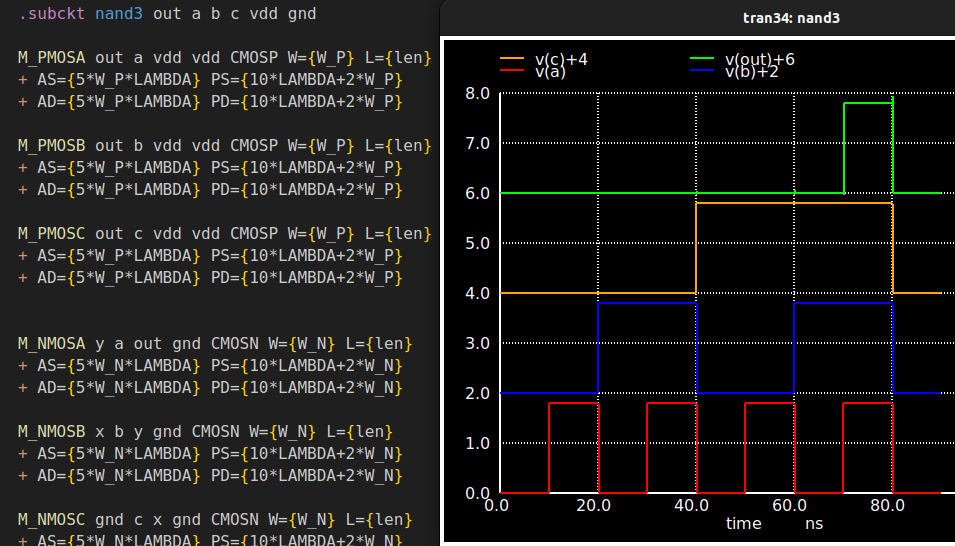
\includegraphics[width=0.4\textwidth]{/home/sudhujoshi/Desktop/Sem_3/VLSI/VLSI_Project/ReportDump/netlist_ss/nand3.png}
    \caption{AND3, Static CMOS Logic} 
\end{figure}
\subsubsection{AND4}
\begin{figure}[H] 
    \centering
    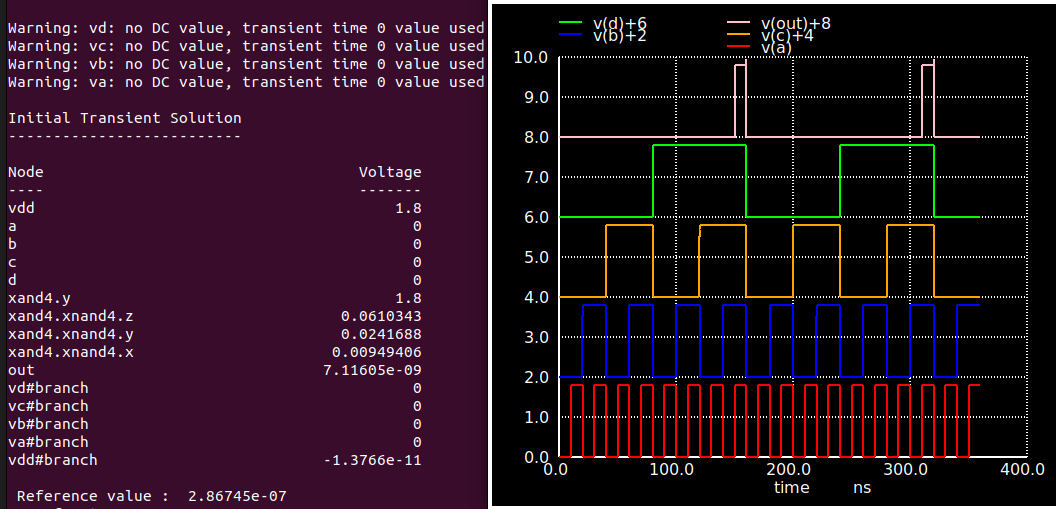
\includegraphics[width=0.4\textwidth]{/home/sudhujoshi/Desktop/Sem_3/VLSI/VLSI_Project/ReportDump/netlist_ss/nand4.png}
    \caption{AND4, Static CMOS Logic} 
\end{figure}
\subsubsection{AND5}
\begin{figure}[H] 
    \centering
    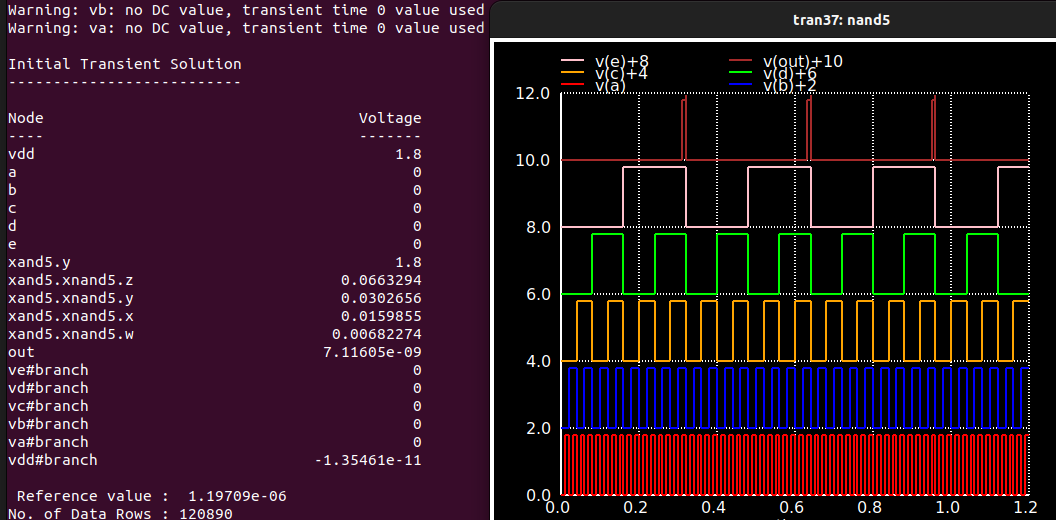
\includegraphics[width=0.4\textwidth]{/home/sudhujoshi/Desktop/Sem_3/VLSI/VLSI_Project/ReportDump/netlist_ss/nand5.png}
    \caption{AND5, Static CMOS Logic} 
\end{figure}

\subsection{OR Logic}
\subsubsection{OR2}
\begin{figure}[H] 
    \centering
    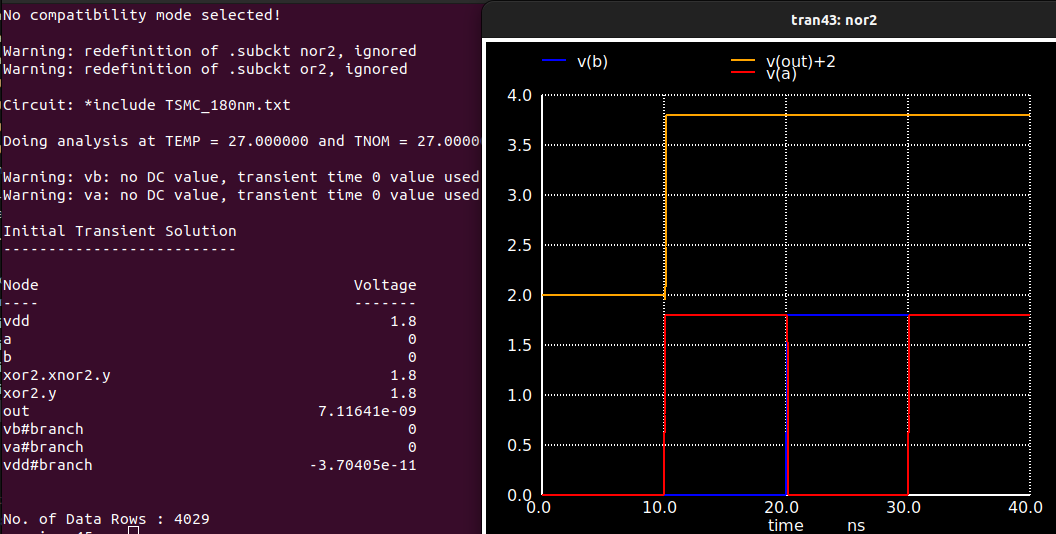
\includegraphics[width=0.4\textwidth]{/home/sudhujoshi/Desktop/Sem_3/VLSI/VLSI_Project/ReportDump/netlist_ss/or2.png}
    \caption{OR2, Static CMOS Logic} 
\end{figure}

\subsubsection{OR3}
\begin{figure}[H] 
    \centering
    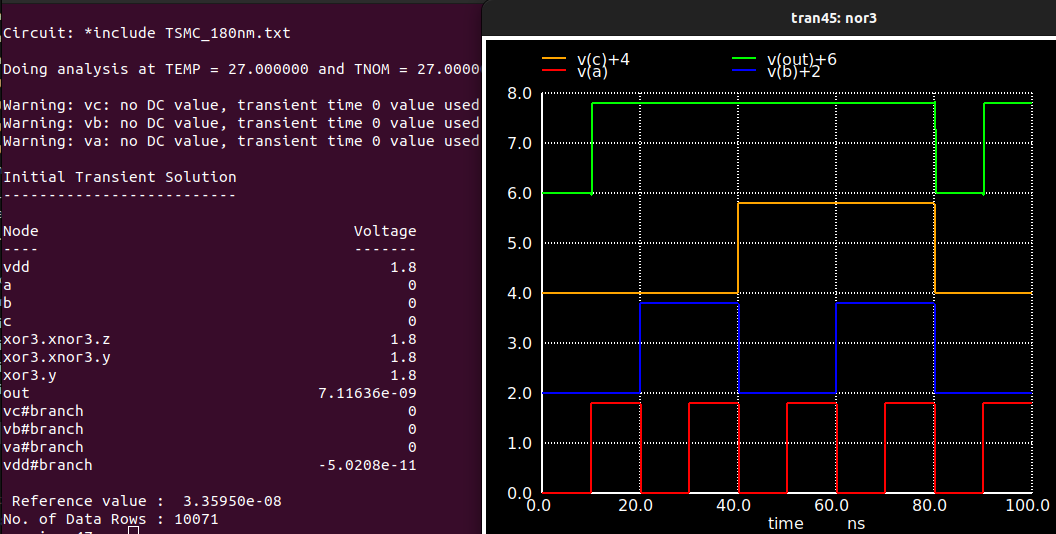
\includegraphics[width=0.4\textwidth]{/home/sudhujoshi/Desktop/Sem_3/VLSI/VLSI_Project/ReportDump/netlist_ss/or3.png}
    \caption{OR3, Static CMOS Logic} 
\end{figure}

\subsubsection{OR4}
\begin{figure}[H]
    \centering
    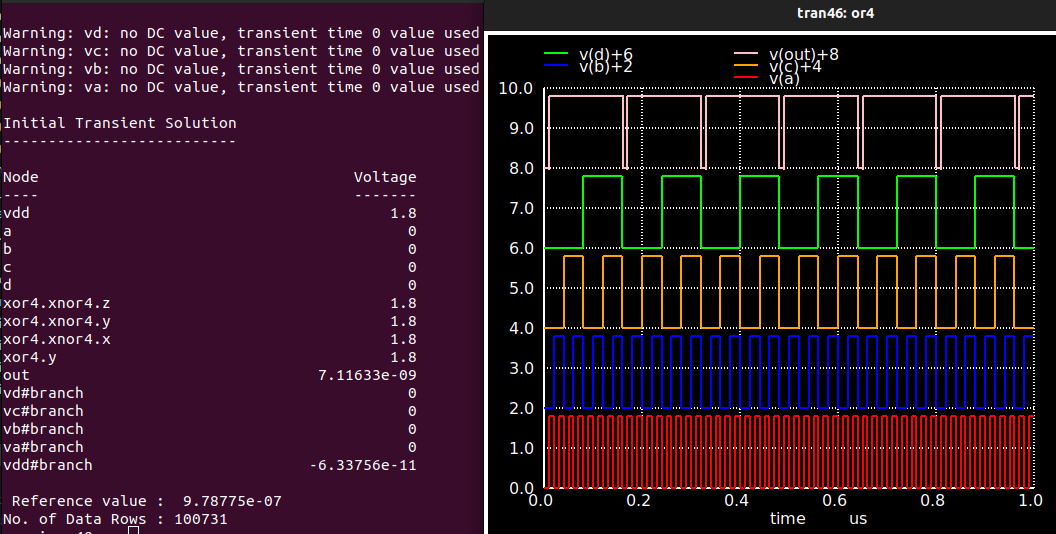
\includegraphics[width=0.4\textwidth]{/home/sudhujoshi/Desktop/Sem_3/VLSI/VLSI_Project/ReportDump/netlist_ss/or4.png}
    \caption{OR4, Static CMOS Logic} 
\end{figure}

\subsubsection{OR5}
\begin{figure}[H]
    \centering
    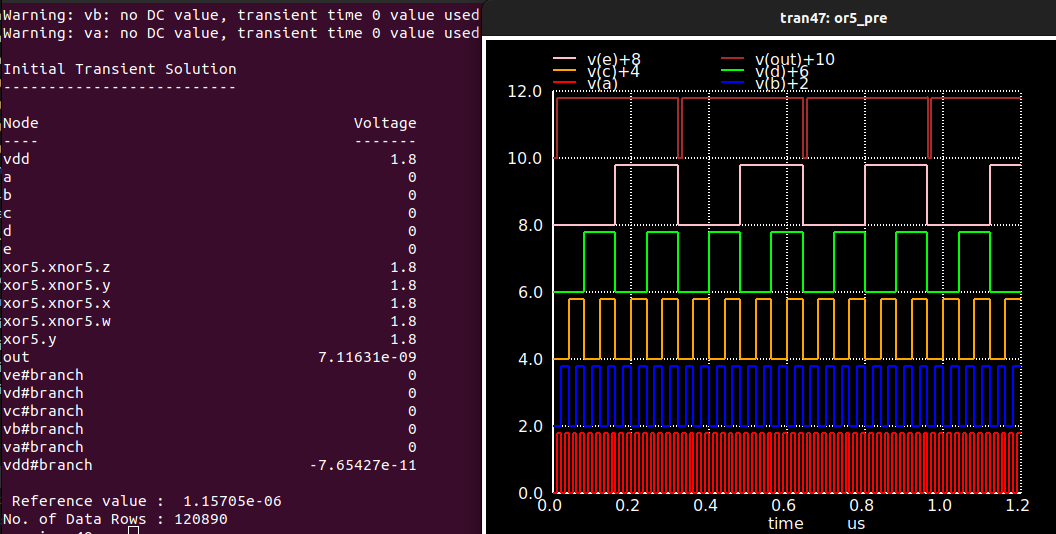
\includegraphics[width=0.4\textwidth]{/home/sudhujoshi/Desktop/Sem_3/VLSI/VLSI_Project/ReportDump/netlist_ss/or5.png}
    \caption{OR5, Static CMOS Logic} 
\end{figure}

\subsection{XOR Logic}
\begin{figure}[H] 
    \centering
    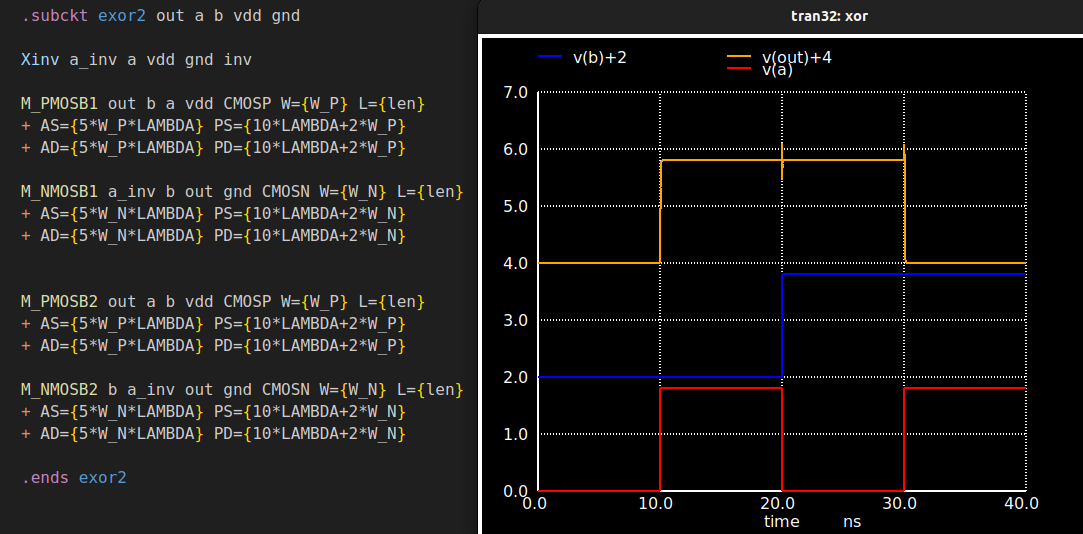
\includegraphics[width=0.375\textwidth]{/home/sudhujoshi/Desktop/Sem_3/VLSI/VLSI_Project/ReportDump/netlist_ss/xor.png}
    \caption{Transmission Gate XOR, NGSpice Netlist}
\end{figure}


\subsection{D Flip-Flop}
\begin{figure}[H] 
    \centering
    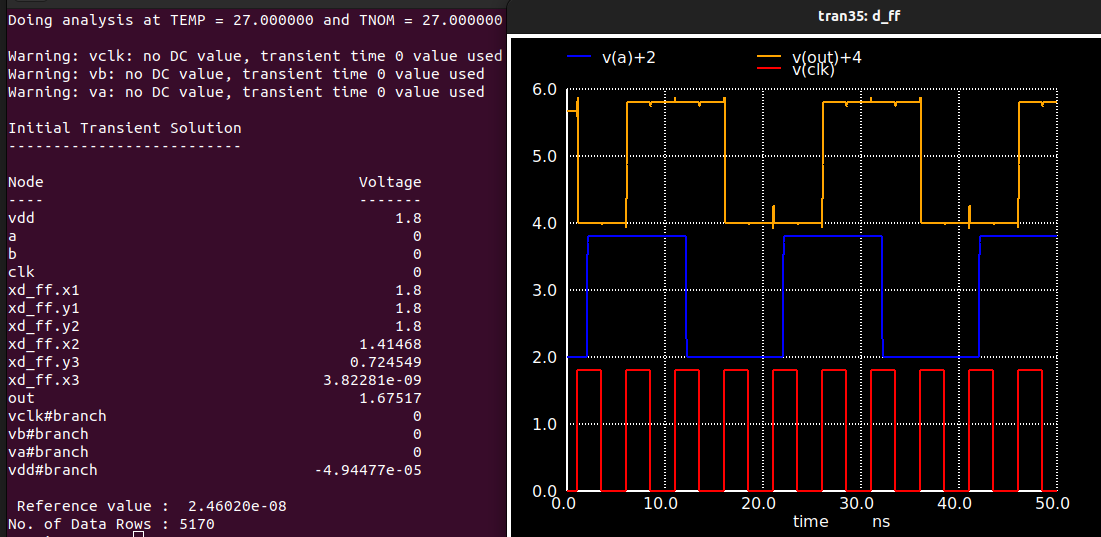
\includegraphics[width=0.4\textwidth]{/home/sudhujoshi/Desktop/Sem_3/VLSI/VLSI_Project/ReportDump/netlist_ss/d_ff.png}
    \caption{TSPC d\_ff, NGSpice Netlist} 
\end{figure}



\section{Setup, Hold, CtQ Time of D\_FF}
For setup, hold and CtQ time delays, the given parameters are found graphically.
% \[
% Fall Time = $0.13388\cdot10^{-9}\;Rise Time = $0.15677\cdot10^{-9}
% \]
\\
Defining \textbf{Clock-to-Q} delay as the time taken for the input change to propagate from the rising edge of the clock to the output \( Q \), we obtain the result through plot observation: 
\[
t_{CtQ} \approx 0.2731\cdot10^{-9}s
\]
\[
t_{prop} \approx 0.20438\cdot10^{-9}s
\]
Given conditions as:
\[
T_{CtQ} + T_{prop} > T_{hold}
\]
\[
\therefore T_{hold} \approx .47748\cdot10^{-9}s
\]

\[
T_{CtQ} + T_{prop} + T_{setup} < T_{TP}
\]
\[
\therefore T_{setup} \approx .41964\cdot10^{-9}s
\]

\begin{figure}[H] 
    \centering
    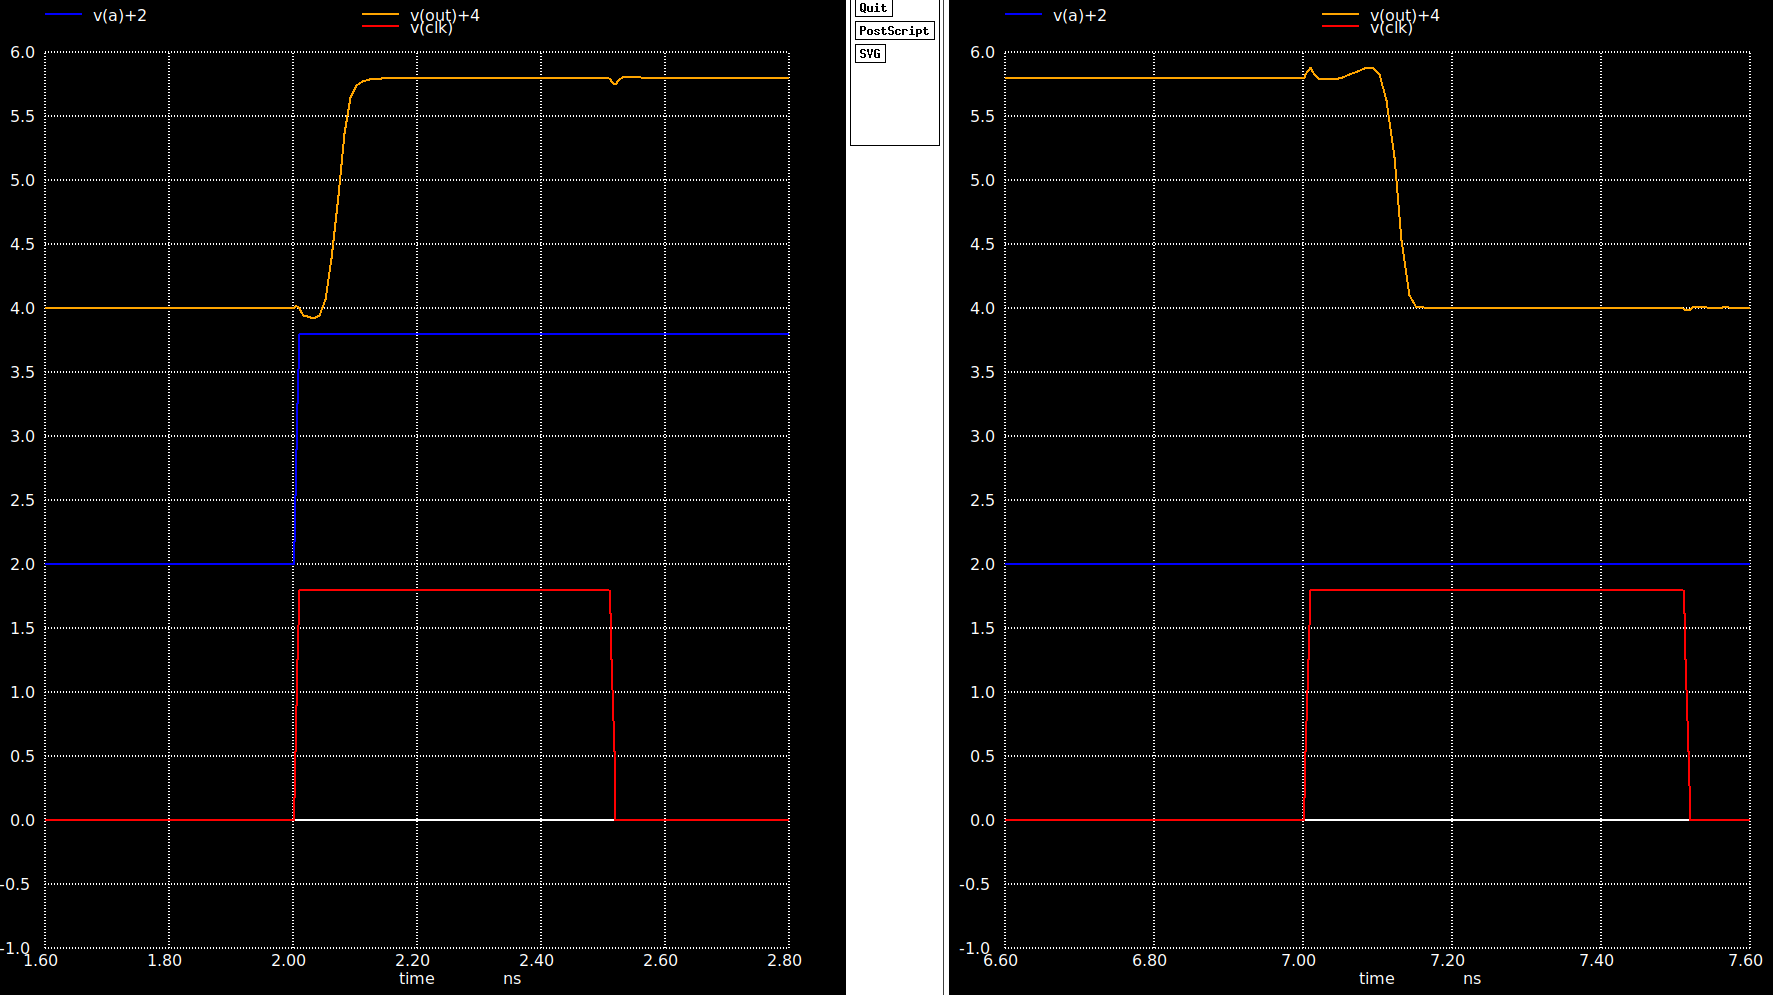
\includegraphics[width=0.4\textwidth]{/home/sudhujoshi/Desktop/Sem_3/VLSI/VLSI_Project/ReportDump/netlist_ss/tcq.png}
    \caption{$Rise\;\&\;Fall$}
\end{figure}

\section{Stick Diagram}
Simplified, abstract representations of CMOS layouts, showing connections without 
exact scaling. They use colored lines to represent polysilicon, metal, and diffusion 
layers, with PMOS transistors placed in the n-well and NMOS transistors in the 
substrate.

\begin{figure}[H] 
    \centering
    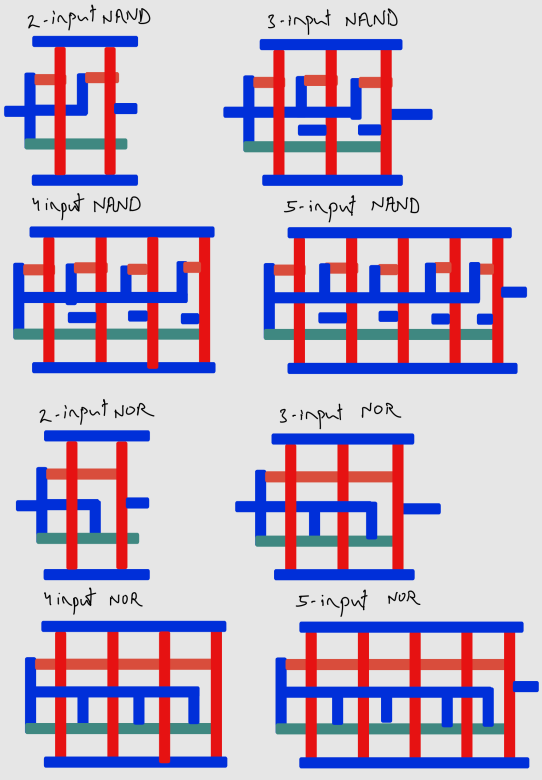
\includegraphics[width=0.3\textwidth]{/home/sudhujoshi/Desktop/Sem_3/VLSI/VLSI_Project/ReportDump/circuit_diagrams/stick.png}
    \caption{Stick Diagrams} 
\end{figure}

\clearpage

\section{MAGIC \& Post-Layout Simulations}

\subsection{AND Logic}
\subsubsection{AND2}
\begin{figure}[H] 
    \centering
    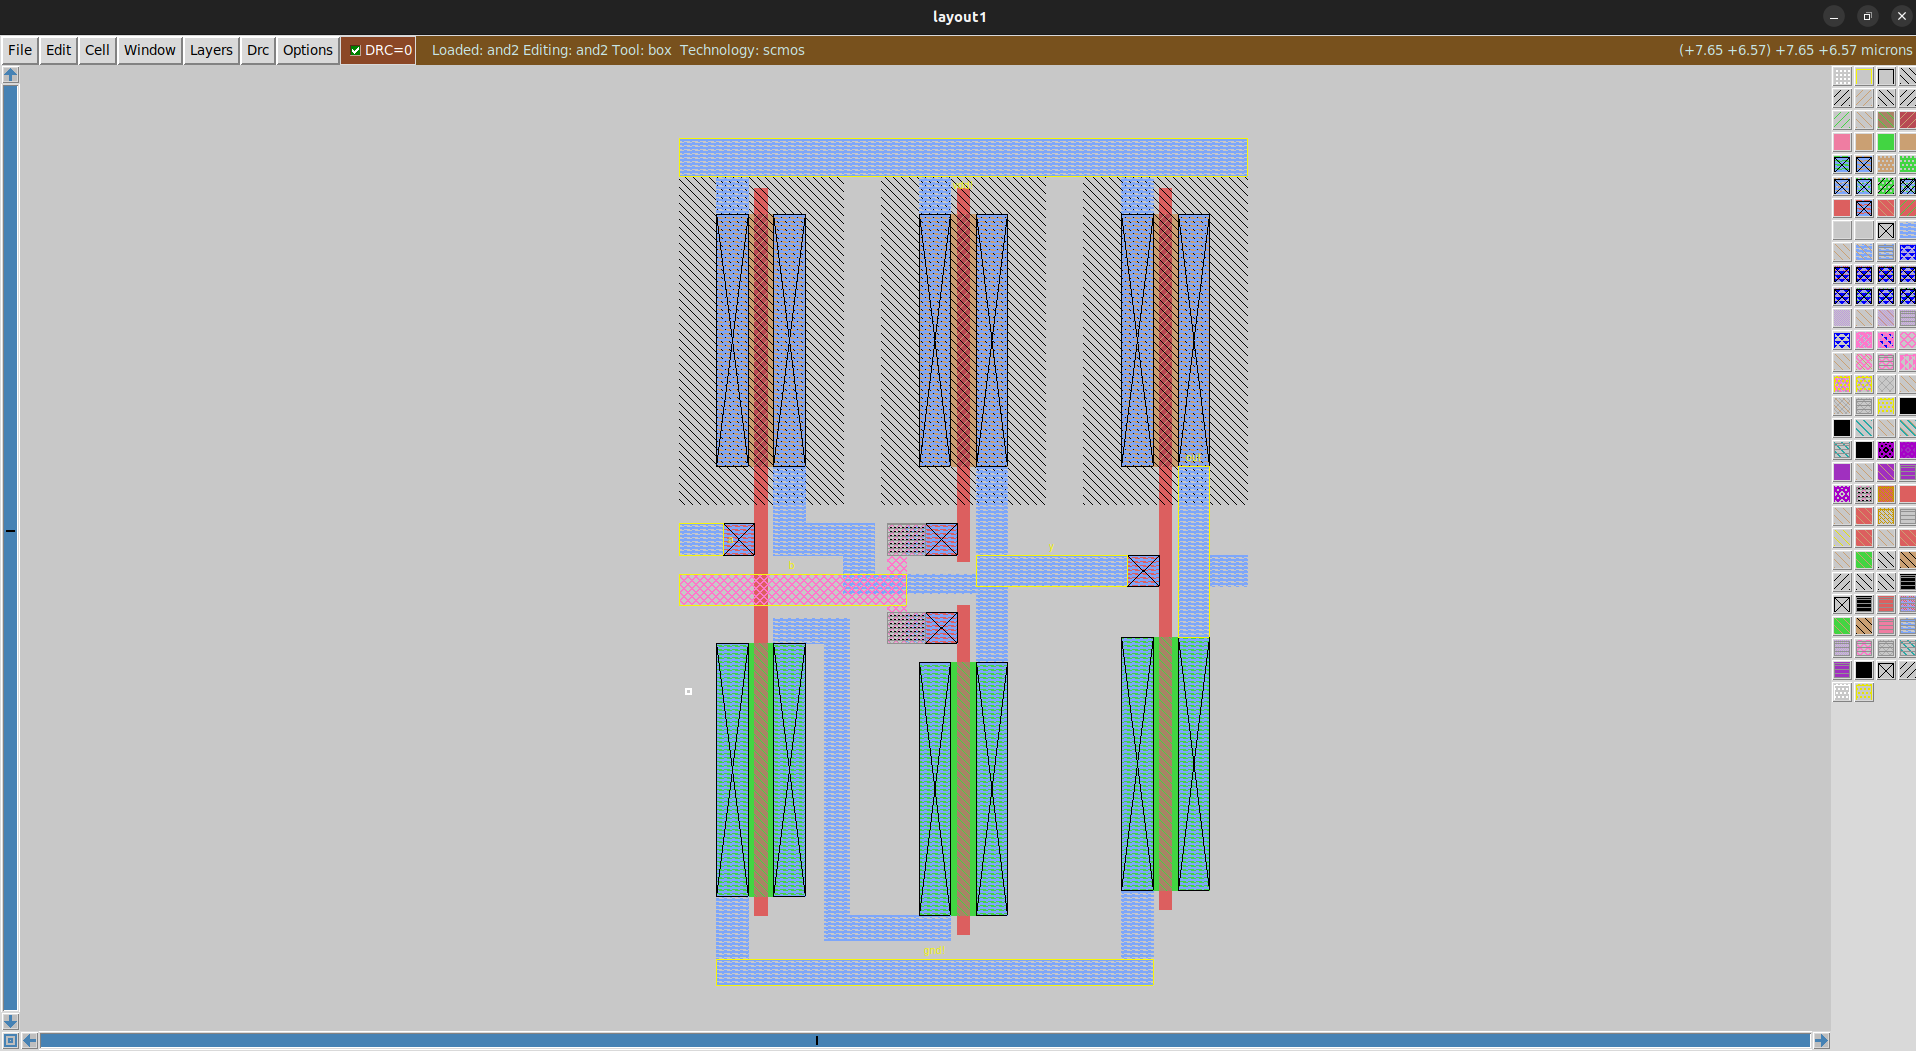
\includegraphics[width=0.375\textwidth]{/home/sudhujoshi/Desktop/Sem_3/VLSI/VLSI_Project/ReportDump/layout_ss/layout_and2.png}
    \caption{MAGIC Layout, AND2} 
\end{figure}

\subsubsection{AND3}
\begin{figure}[H] 
    \centering
    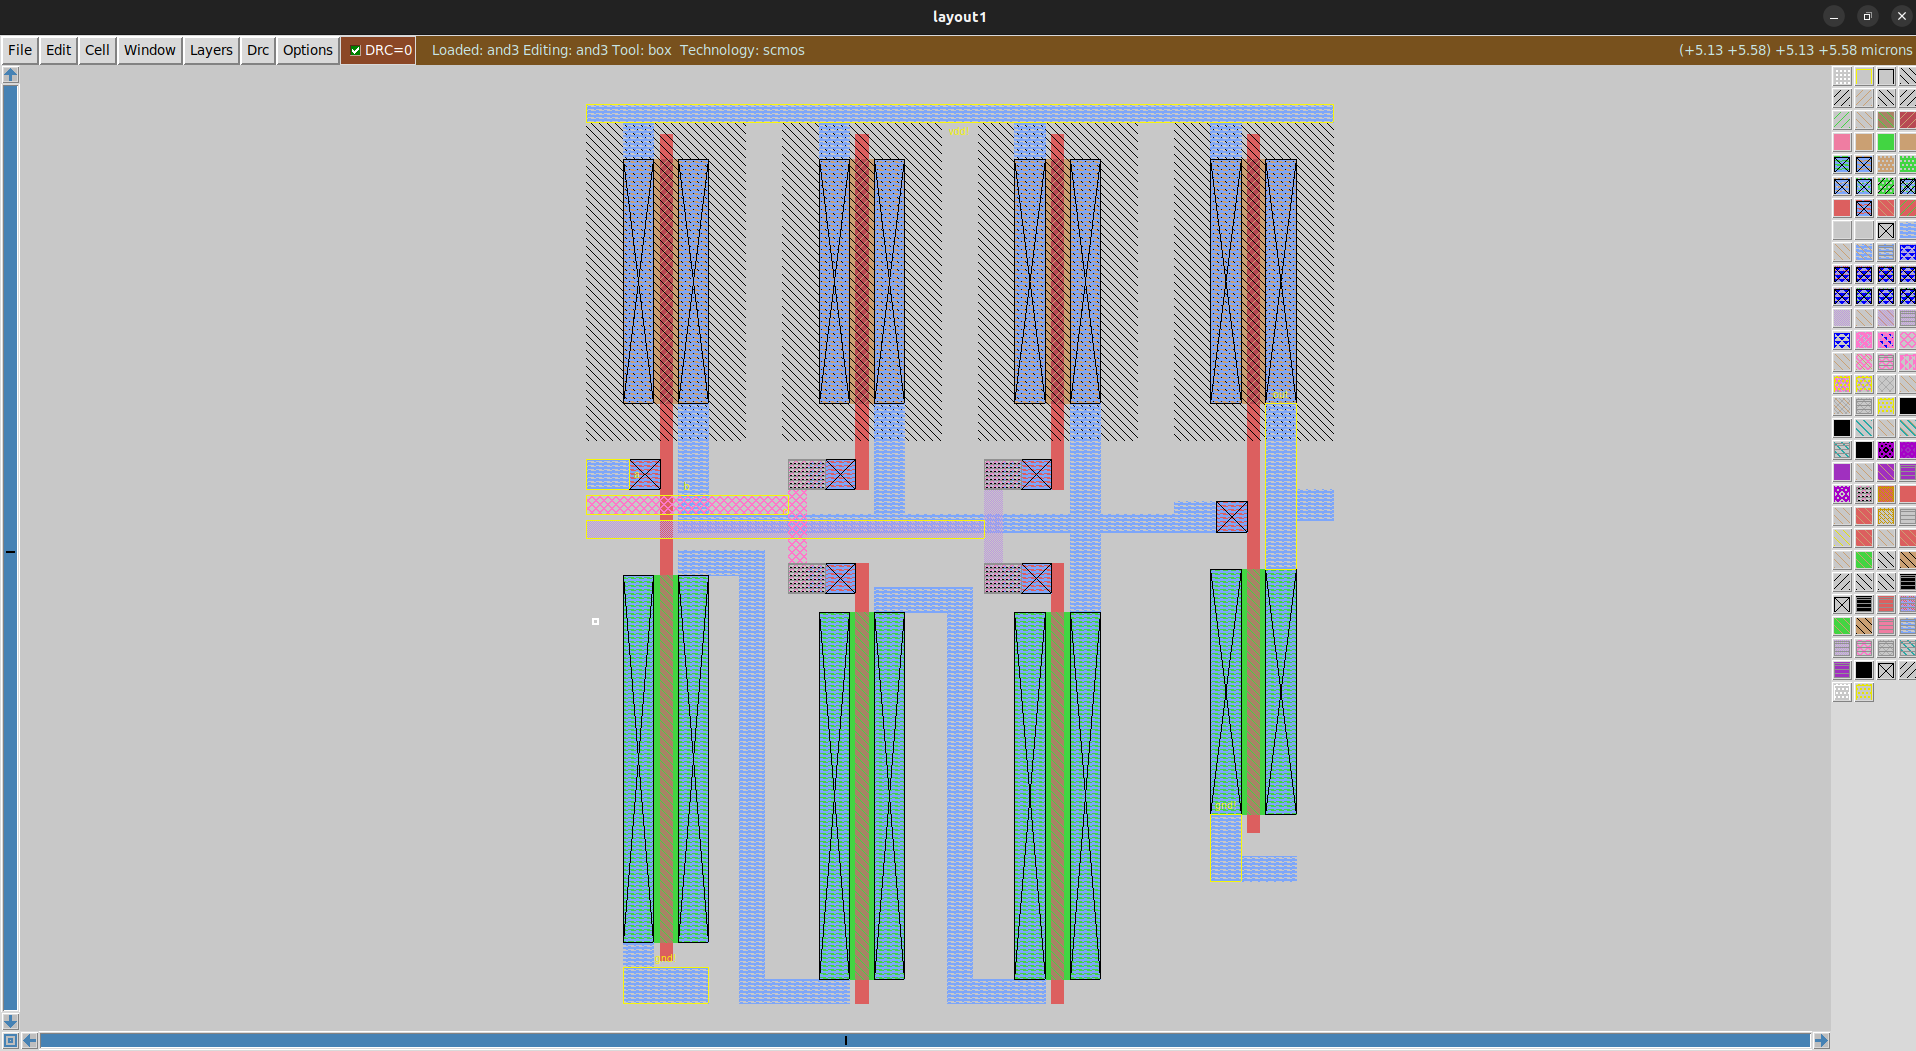
\includegraphics[width=0.375\textwidth]{/home/sudhujoshi/Desktop/Sem_3/VLSI/VLSI_Project/ReportDump/layout_ss/layout_and3.png}
    \caption{MAGIC Layout, AND3} 
\end{figure}

\subsubsection{AND4}
\begin{figure}[H] 
    \centering
    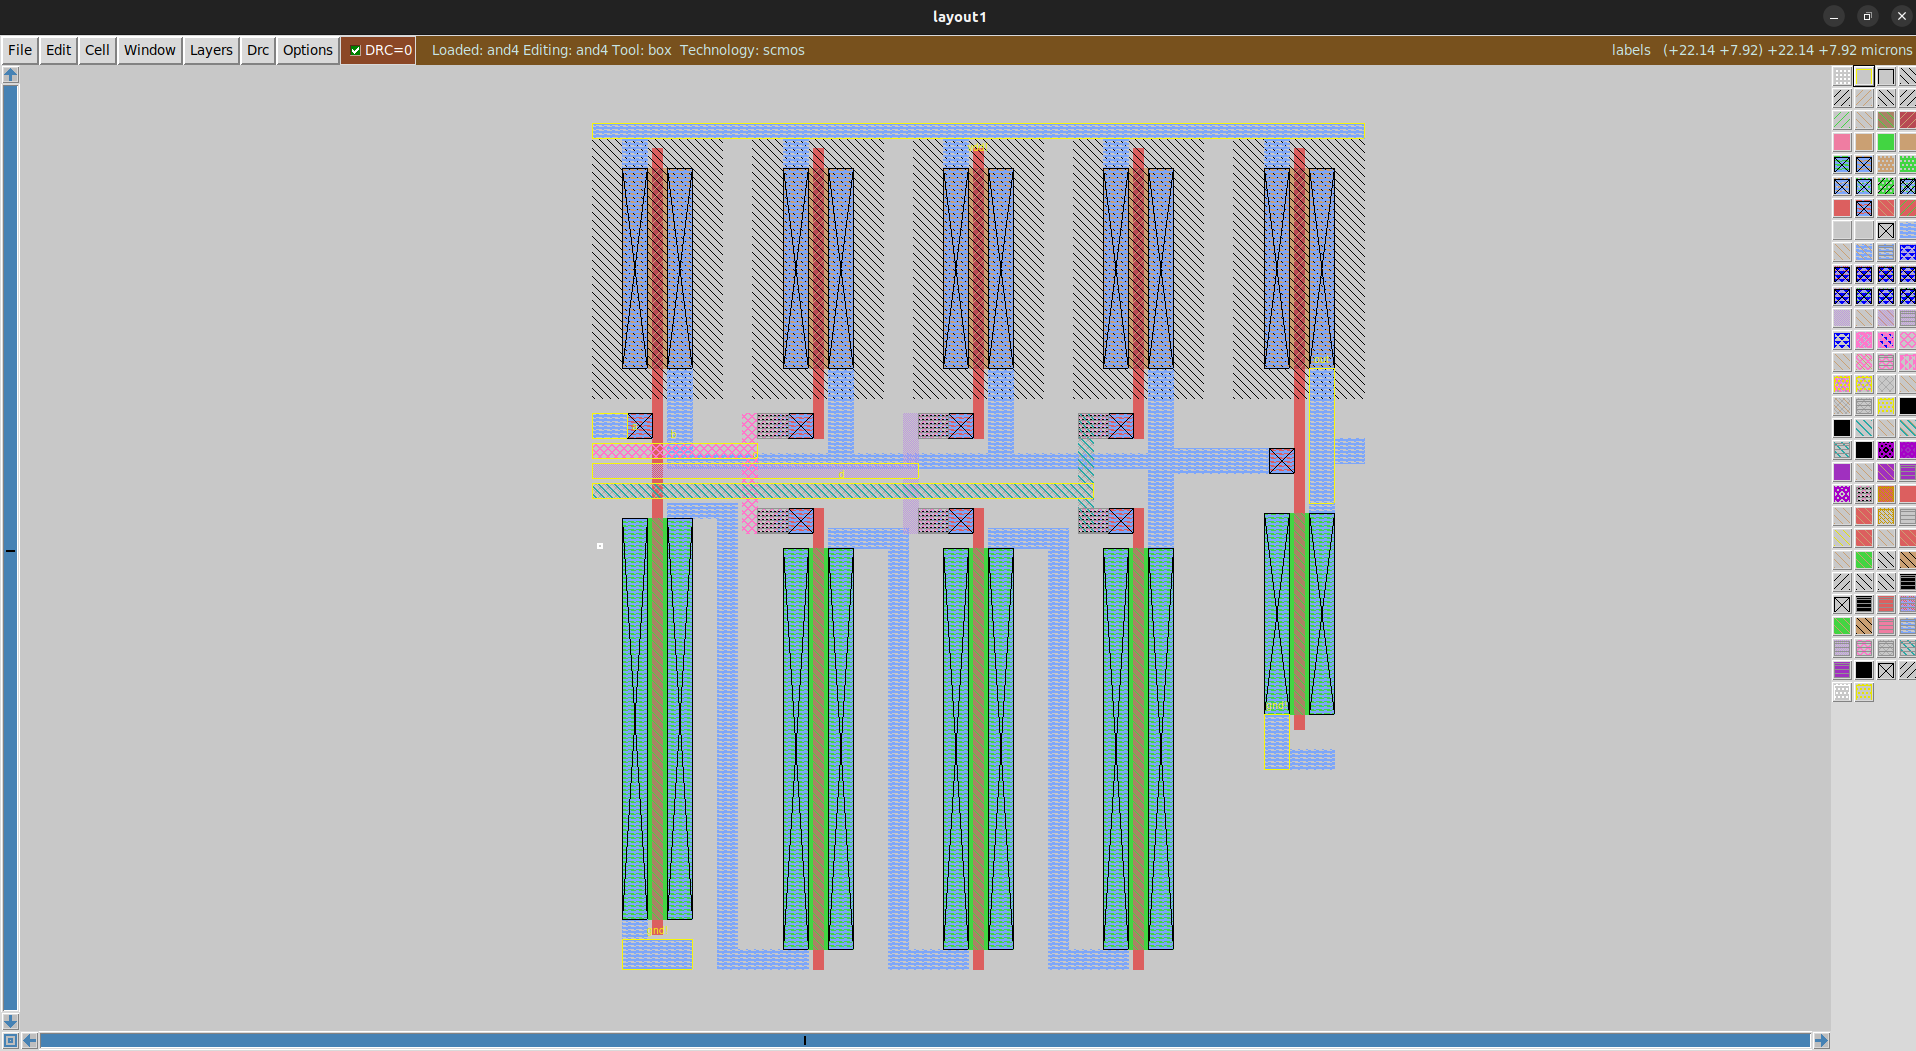
\includegraphics[width=0.375\textwidth]{/home/sudhujoshi/Desktop/Sem_3/VLSI/VLSI_Project/ReportDump/layout_ss/layout_and4.png}
    \caption{MAGIC Layout, AND4} 
\end{figure}

\subsubsection{AND5}
\begin{figure}[H] 
    \centering
    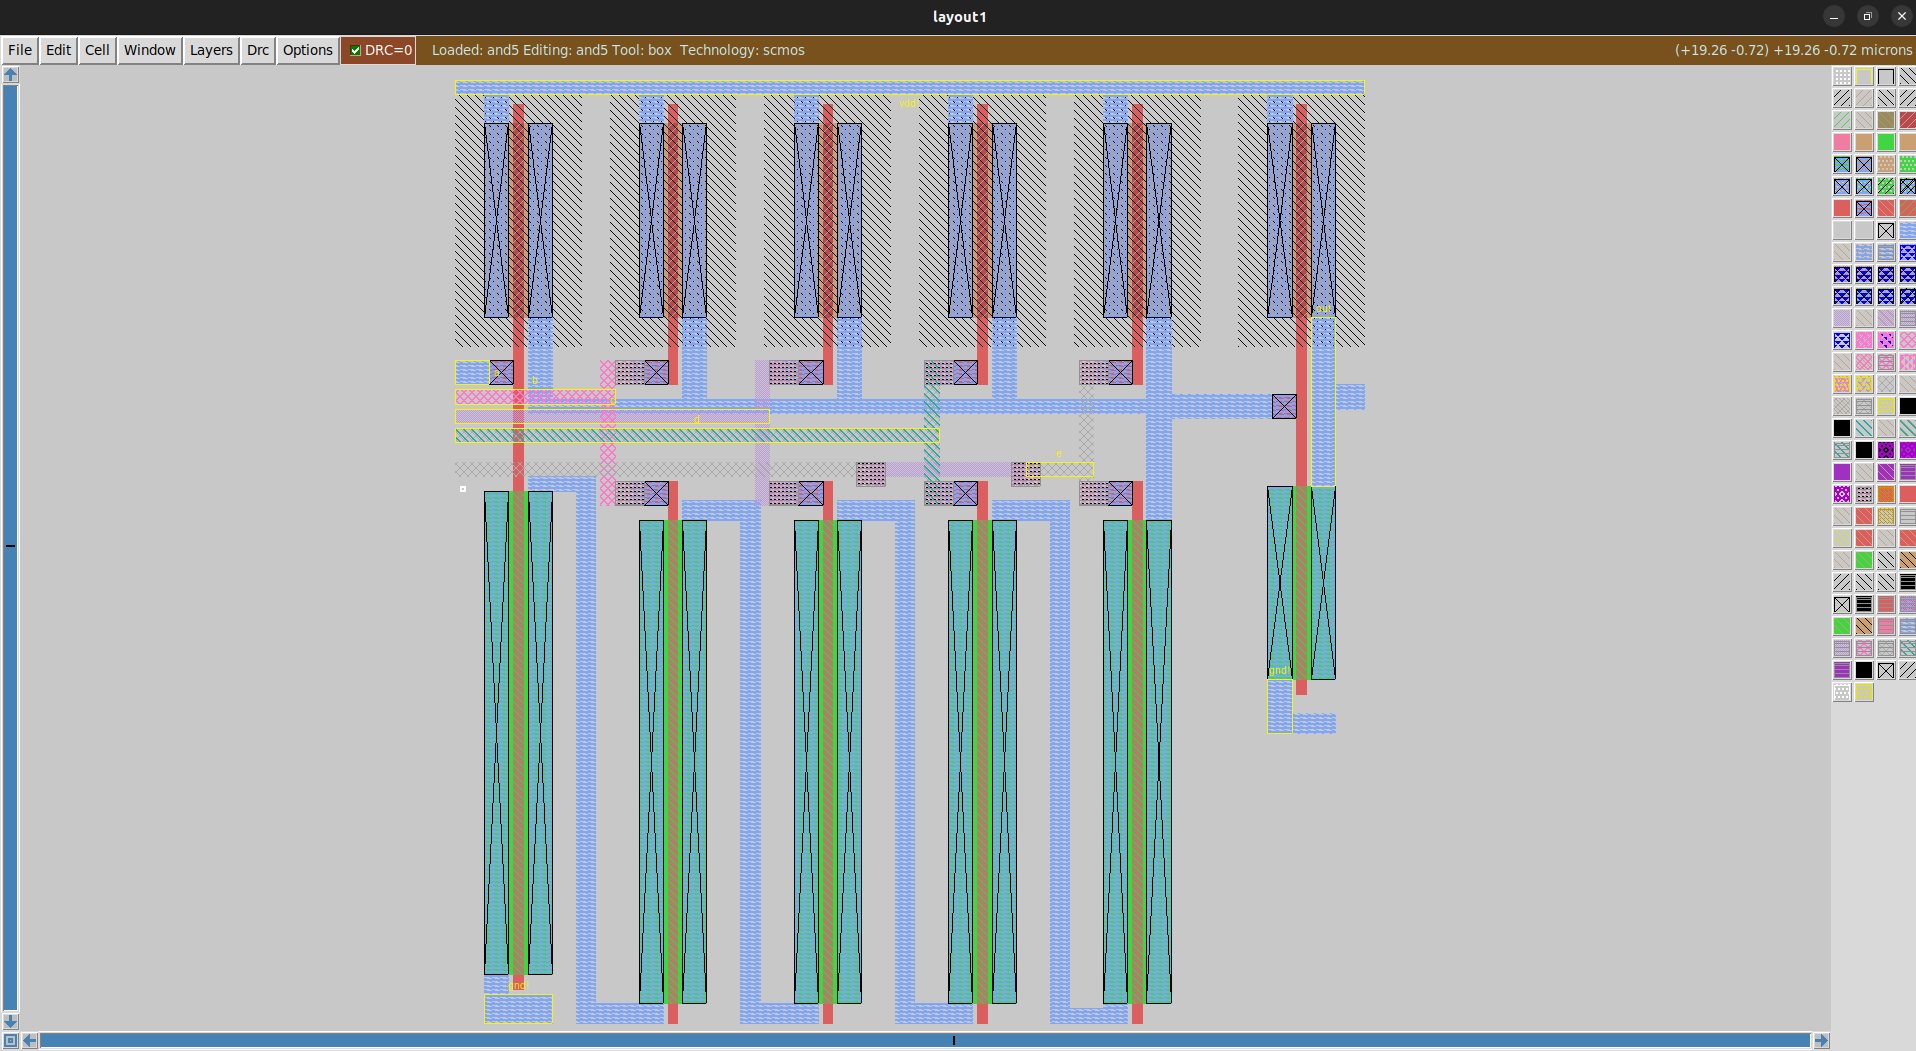
\includegraphics[width=0.375\textwidth]{/home/sudhujoshi/Desktop/Sem_3/VLSI/VLSI_Project/ReportDump/layout_ss/layout_and5.png}
    \caption{MAGIC Layout, AND5} 
\end{figure}

\subsection{OR Logic}
\subsubsection{OR2}
\begin{figure}[H] 
    \centering
    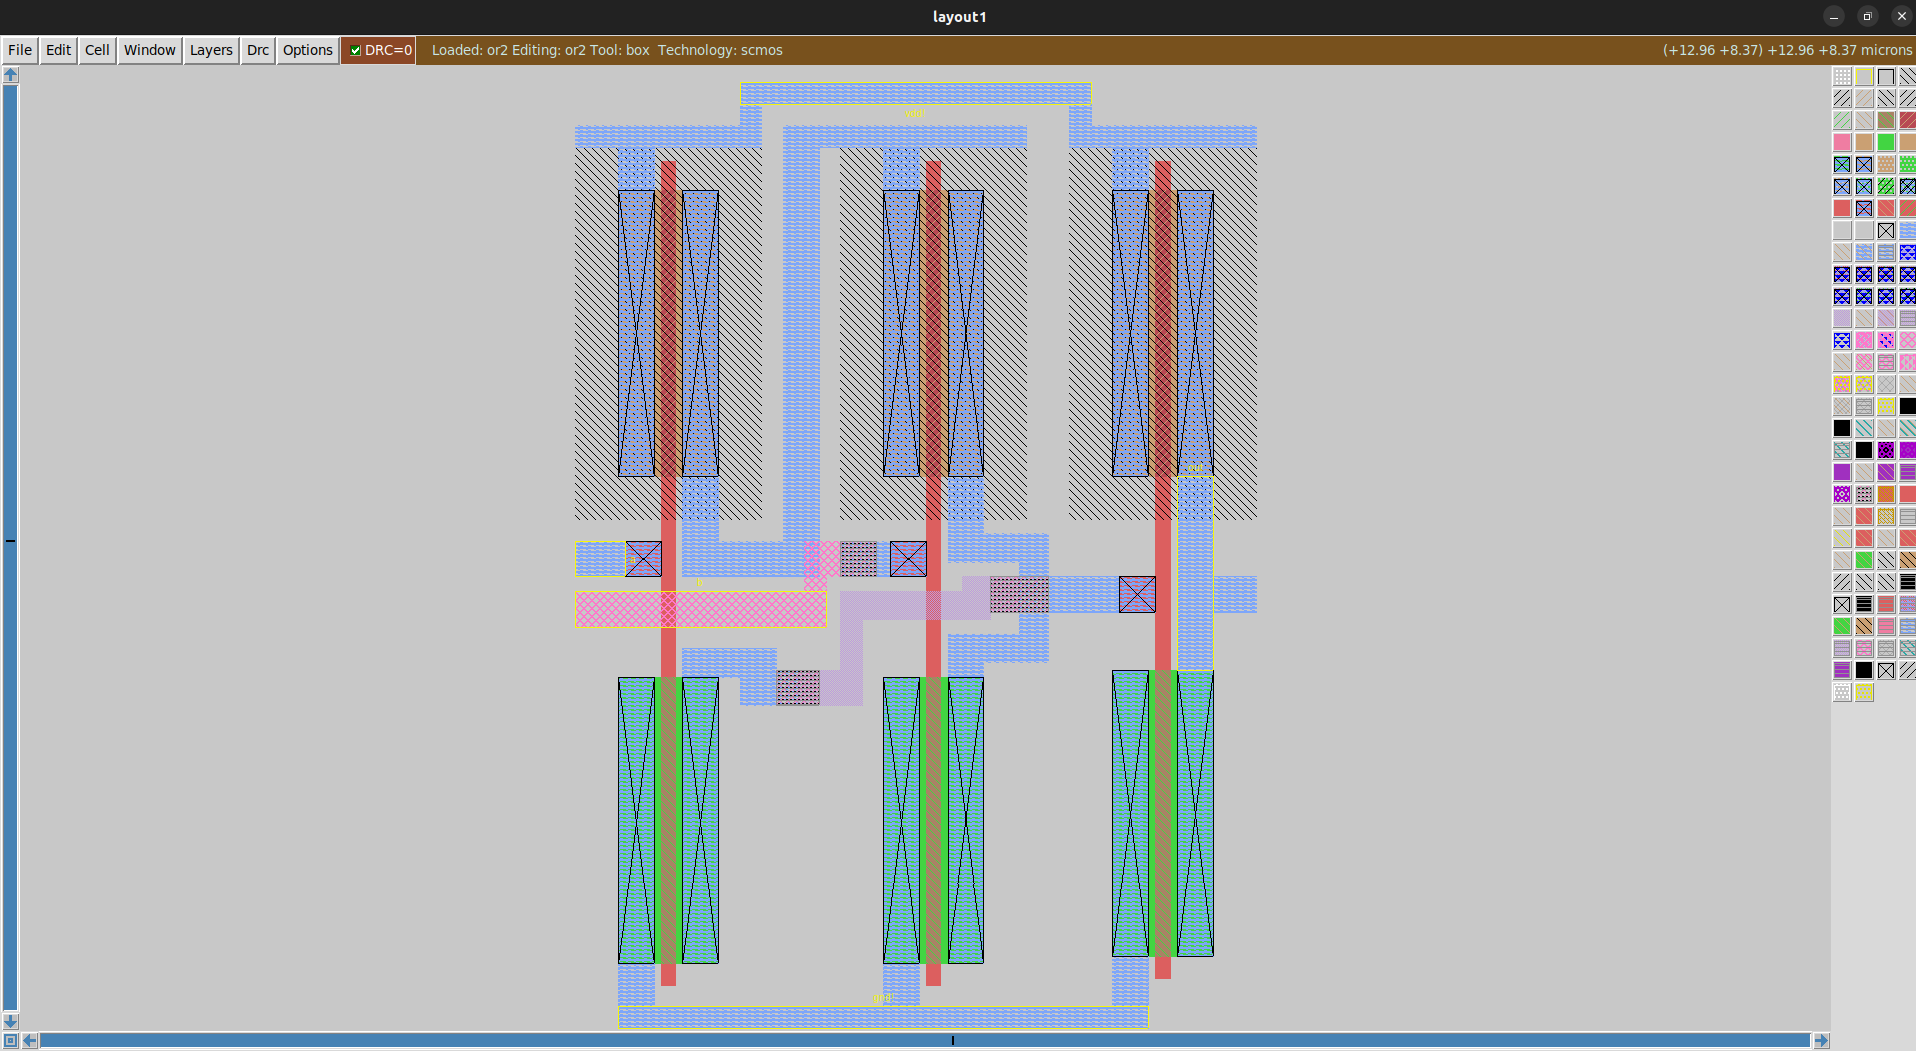
\includegraphics[width=0.375\textwidth]{/home/sudhujoshi/Desktop/Sem_3/VLSI/VLSI_Project/ReportDump/layout_ss/layout_or2.png}
    \caption{MAGIC Layout, OR2} 
\end{figure}
\subsubsection{OR3}
\begin{figure}[H] 
    \centering
    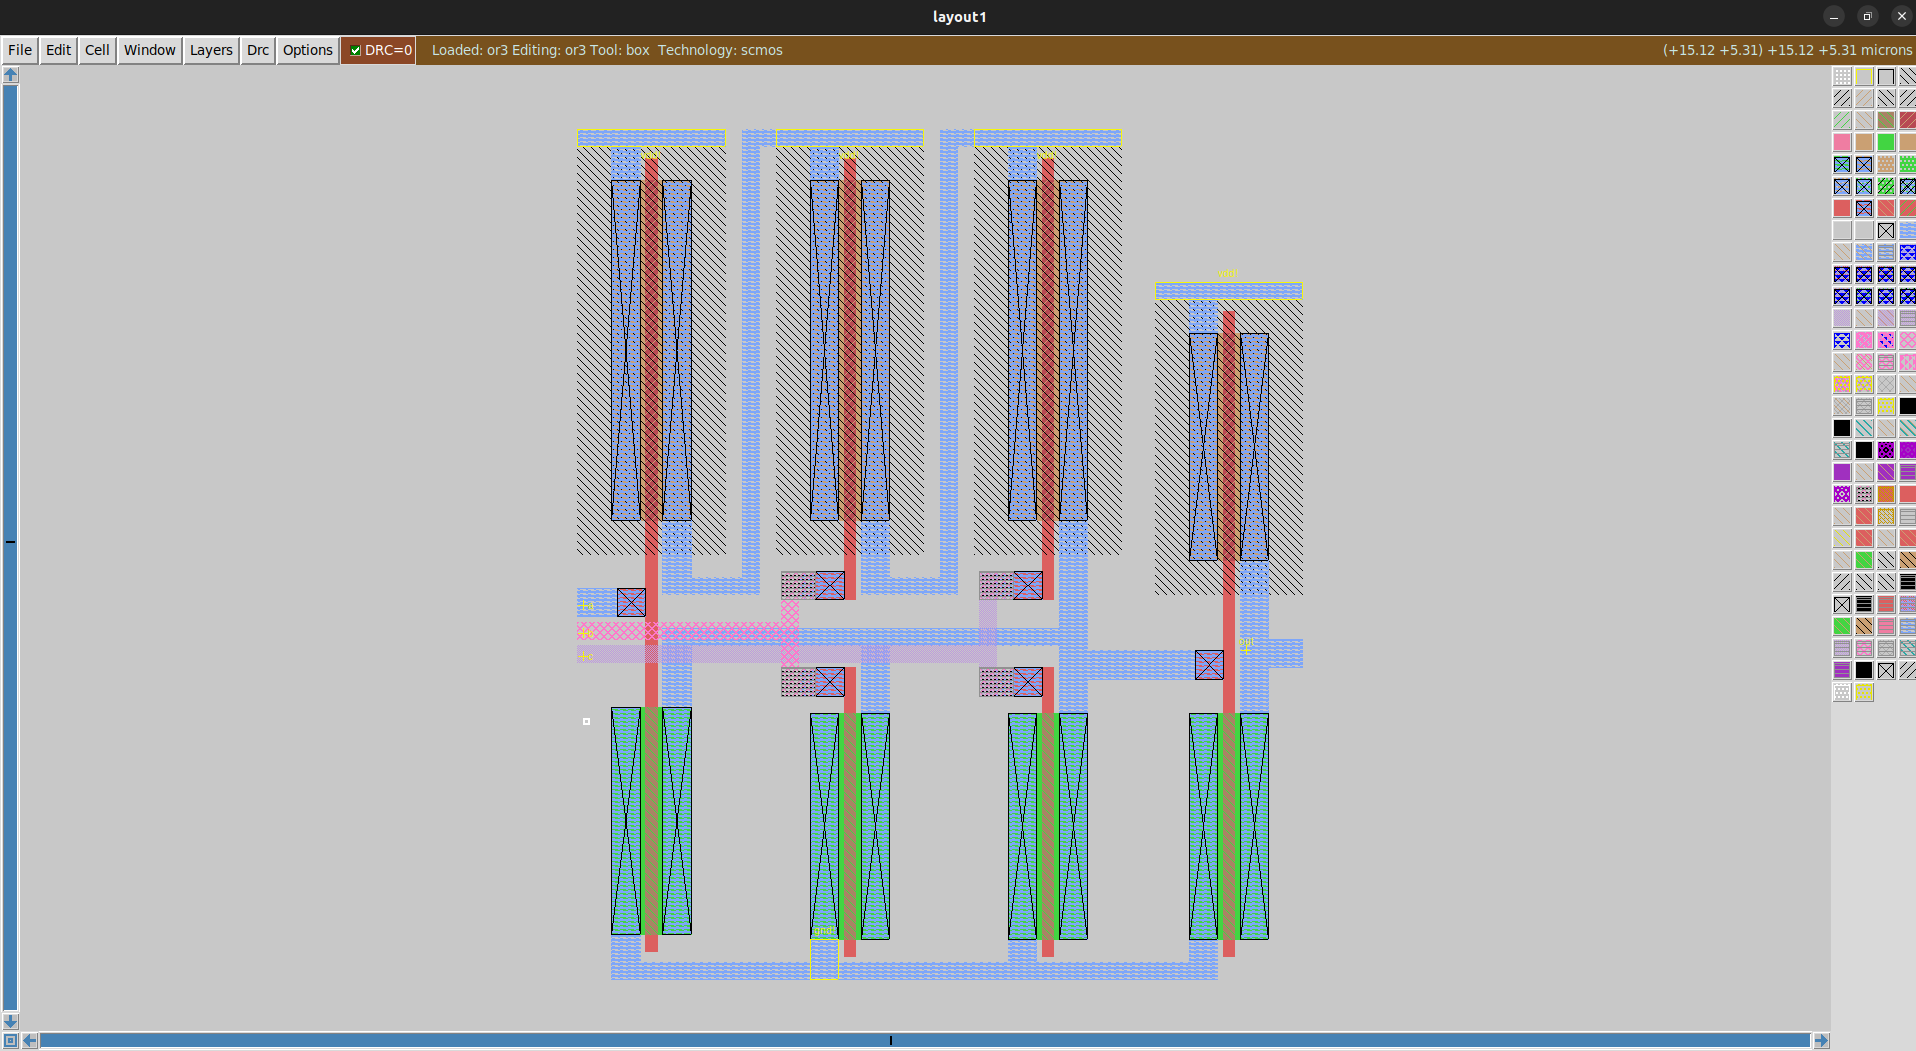
\includegraphics[width=0.375\textwidth]{/home/sudhujoshi/Desktop/Sem_3/VLSI/VLSI_Project/ReportDump/layout_ss/layout_or3.png}
    \caption{MAGIC Layout, OR3} 
\end{figure}
\subsubsection{OR4}
\begin{figure}[H] 
    \centering
    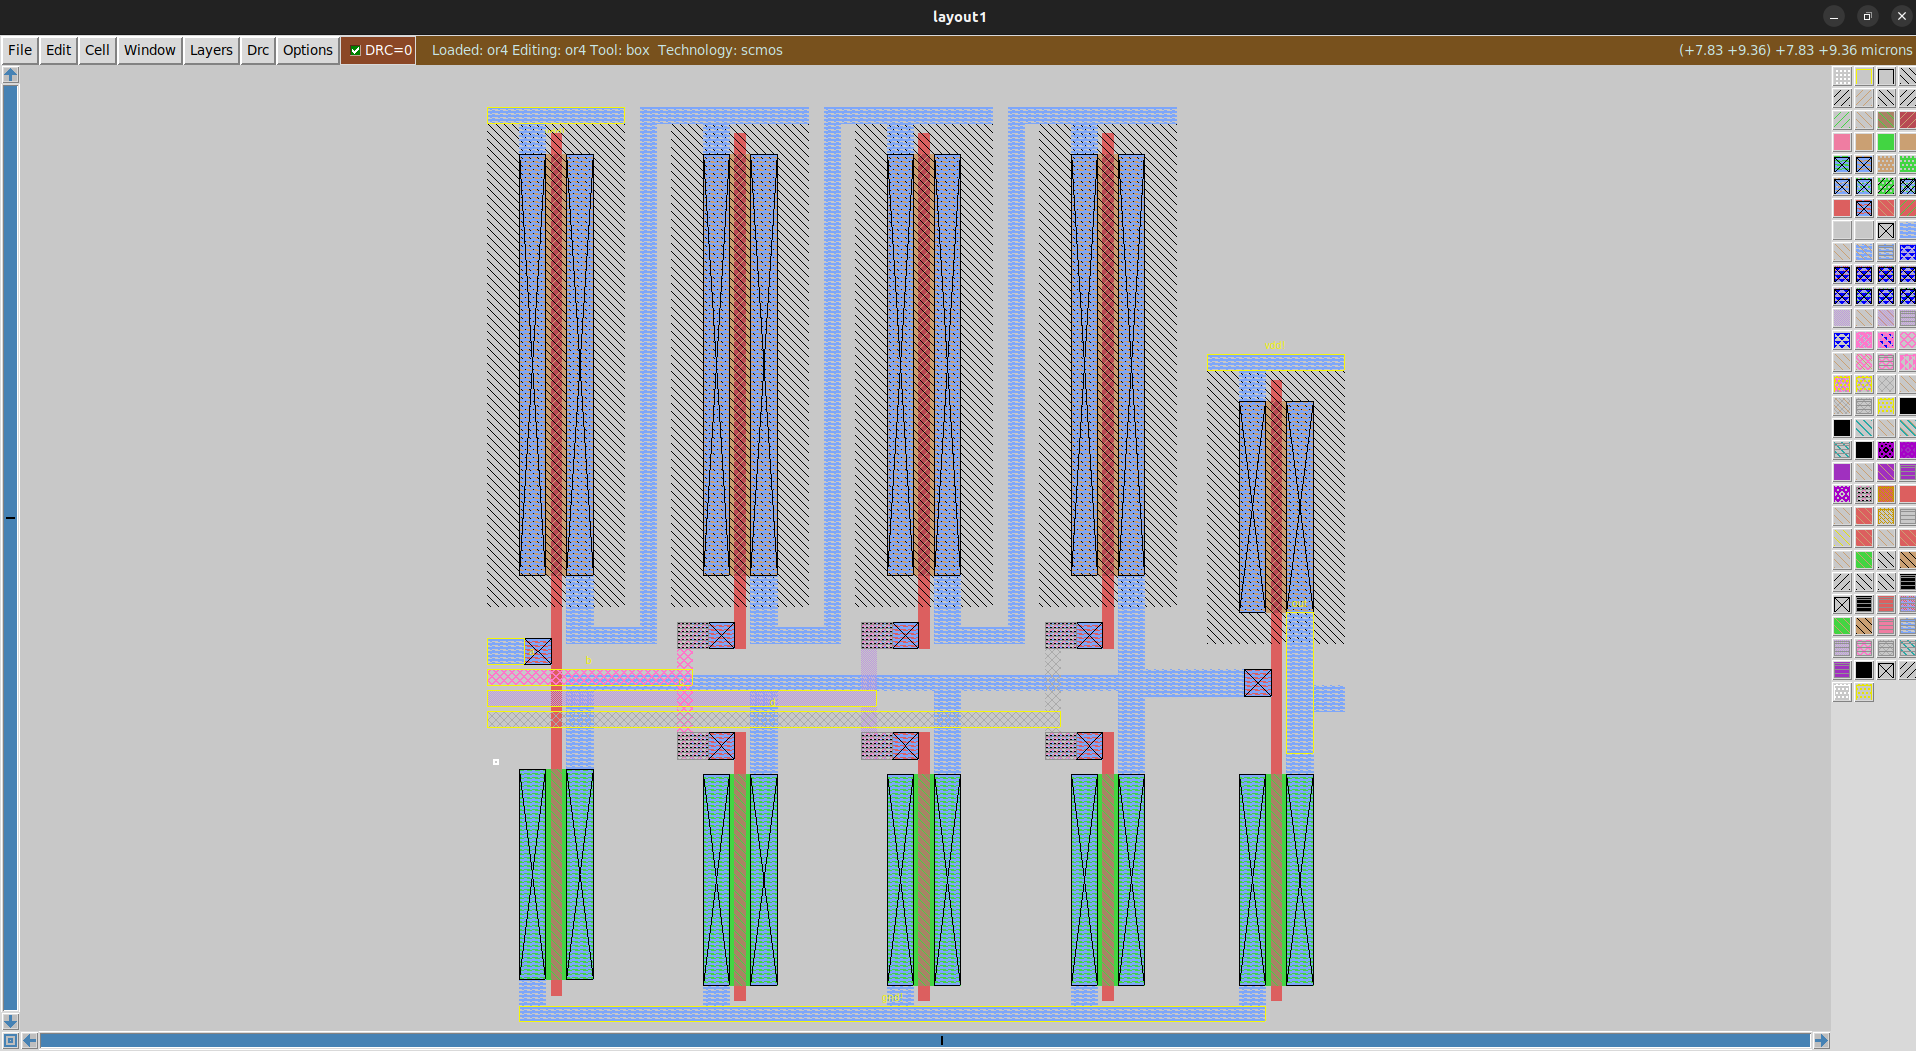
\includegraphics[width=0.375\textwidth]{/home/sudhujoshi/Desktop/Sem_3/VLSI/VLSI_Project/ReportDump/layout_ss/layout_or4.png}
    \caption{MAGIC Layout, OR4} 
\end{figure}
\subsubsection{OR5}
\begin{figure}[H] 
    \centering
    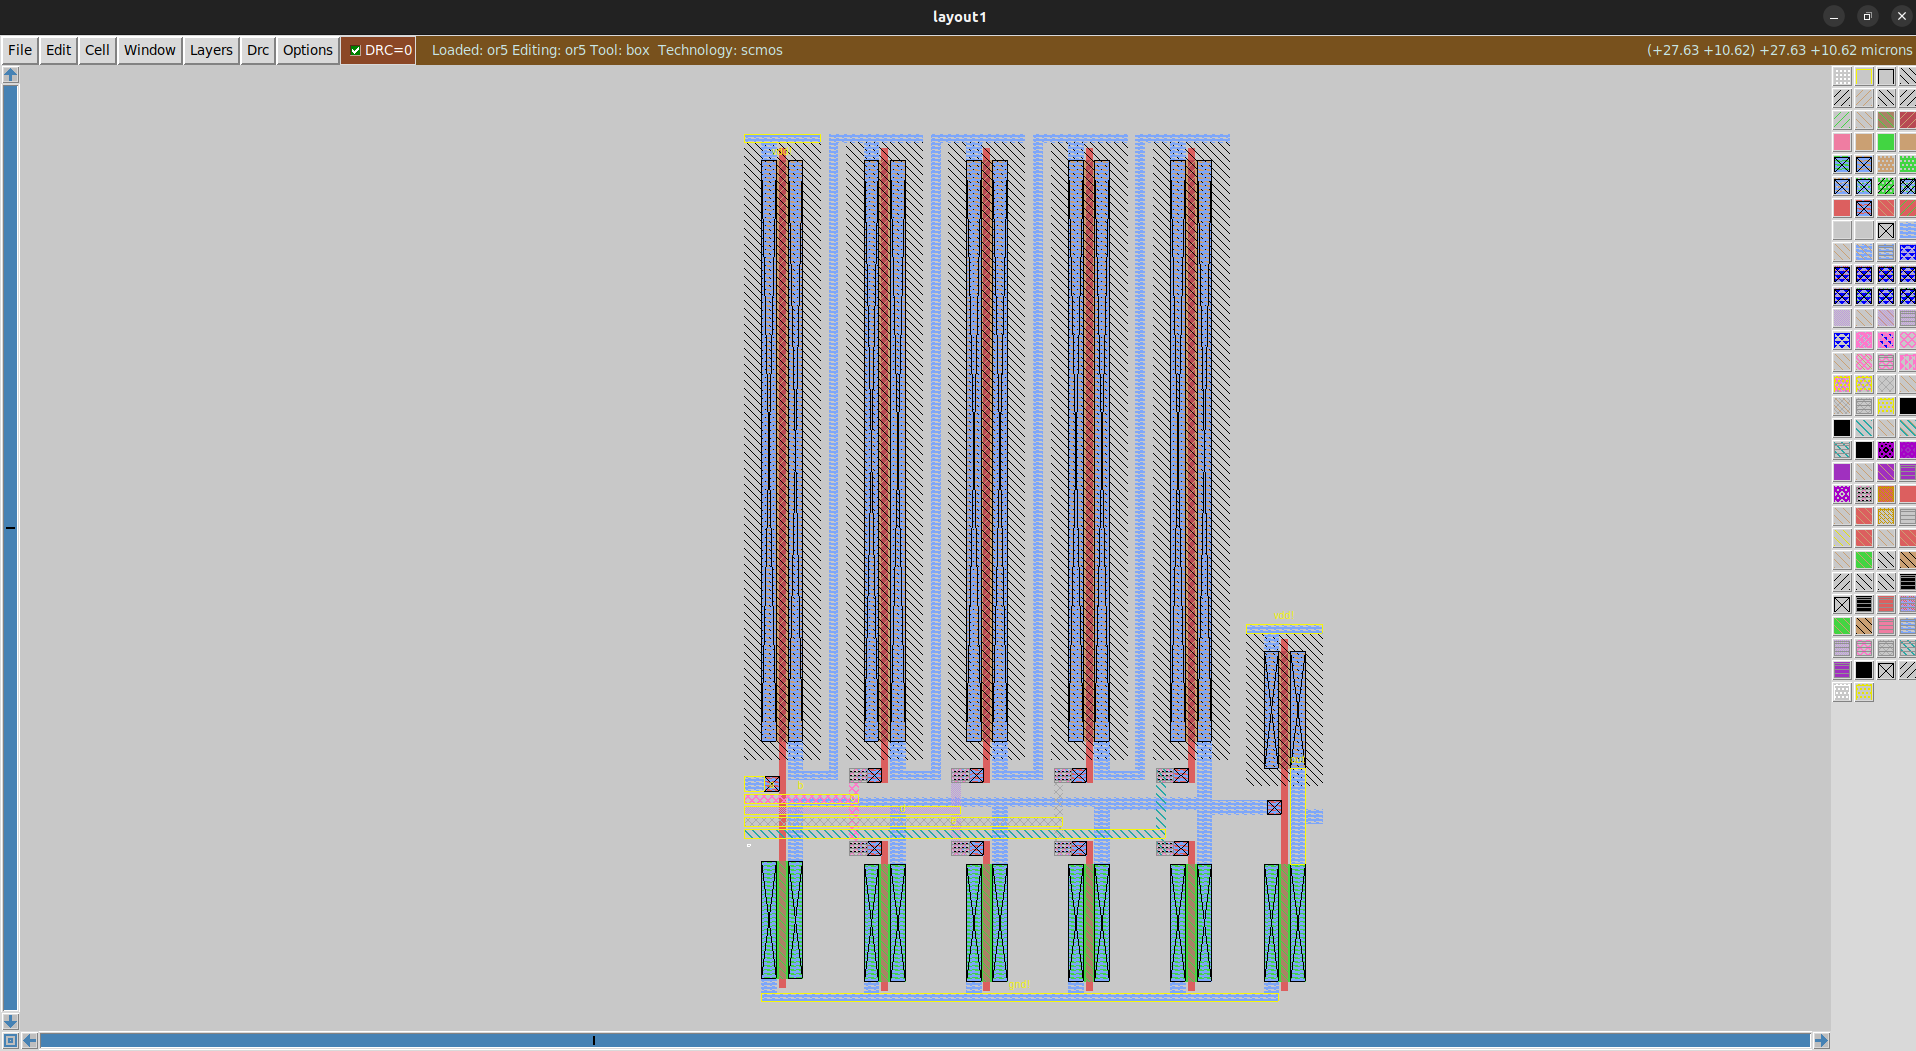
\includegraphics[width=0.375\textwidth]{/home/sudhujoshi/Desktop/Sem_3/VLSI/VLSI_Project/ReportDump/layout_ss/layout_or5.png}
    \caption{MAGIC Layout, OR5} 
\end{figure}


\subsection{XOR Logic}
\begin{figure}[H] 
    \centering
    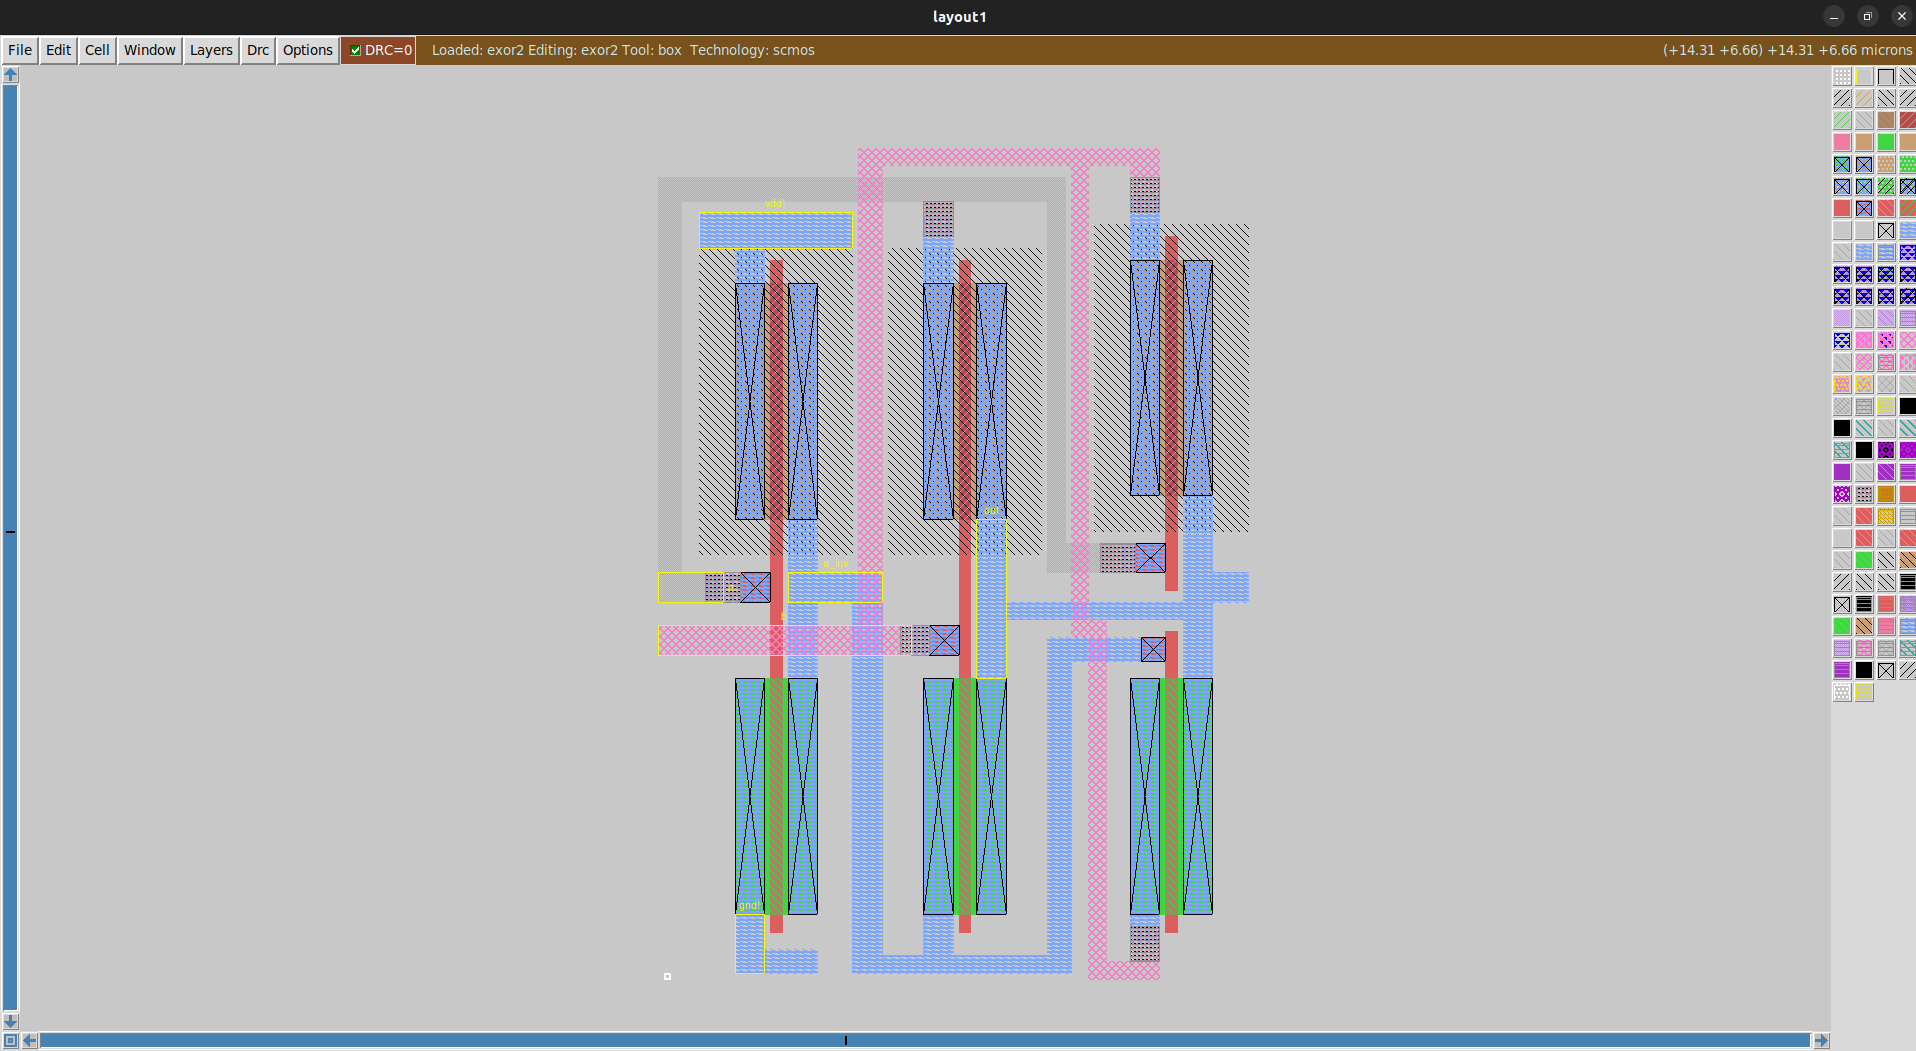
\includegraphics[width=0.45\textwidth]{/home/sudhujoshi/Desktop/Sem_3/VLSI/VLSI_Project/ReportDump/layout_ss/layout_exor.png}
    \caption{MAGIC Layout, XOR} 
\end{figure}

\subsection{D Flip-Flop}
\begin{figure}[H] 
    \centering
    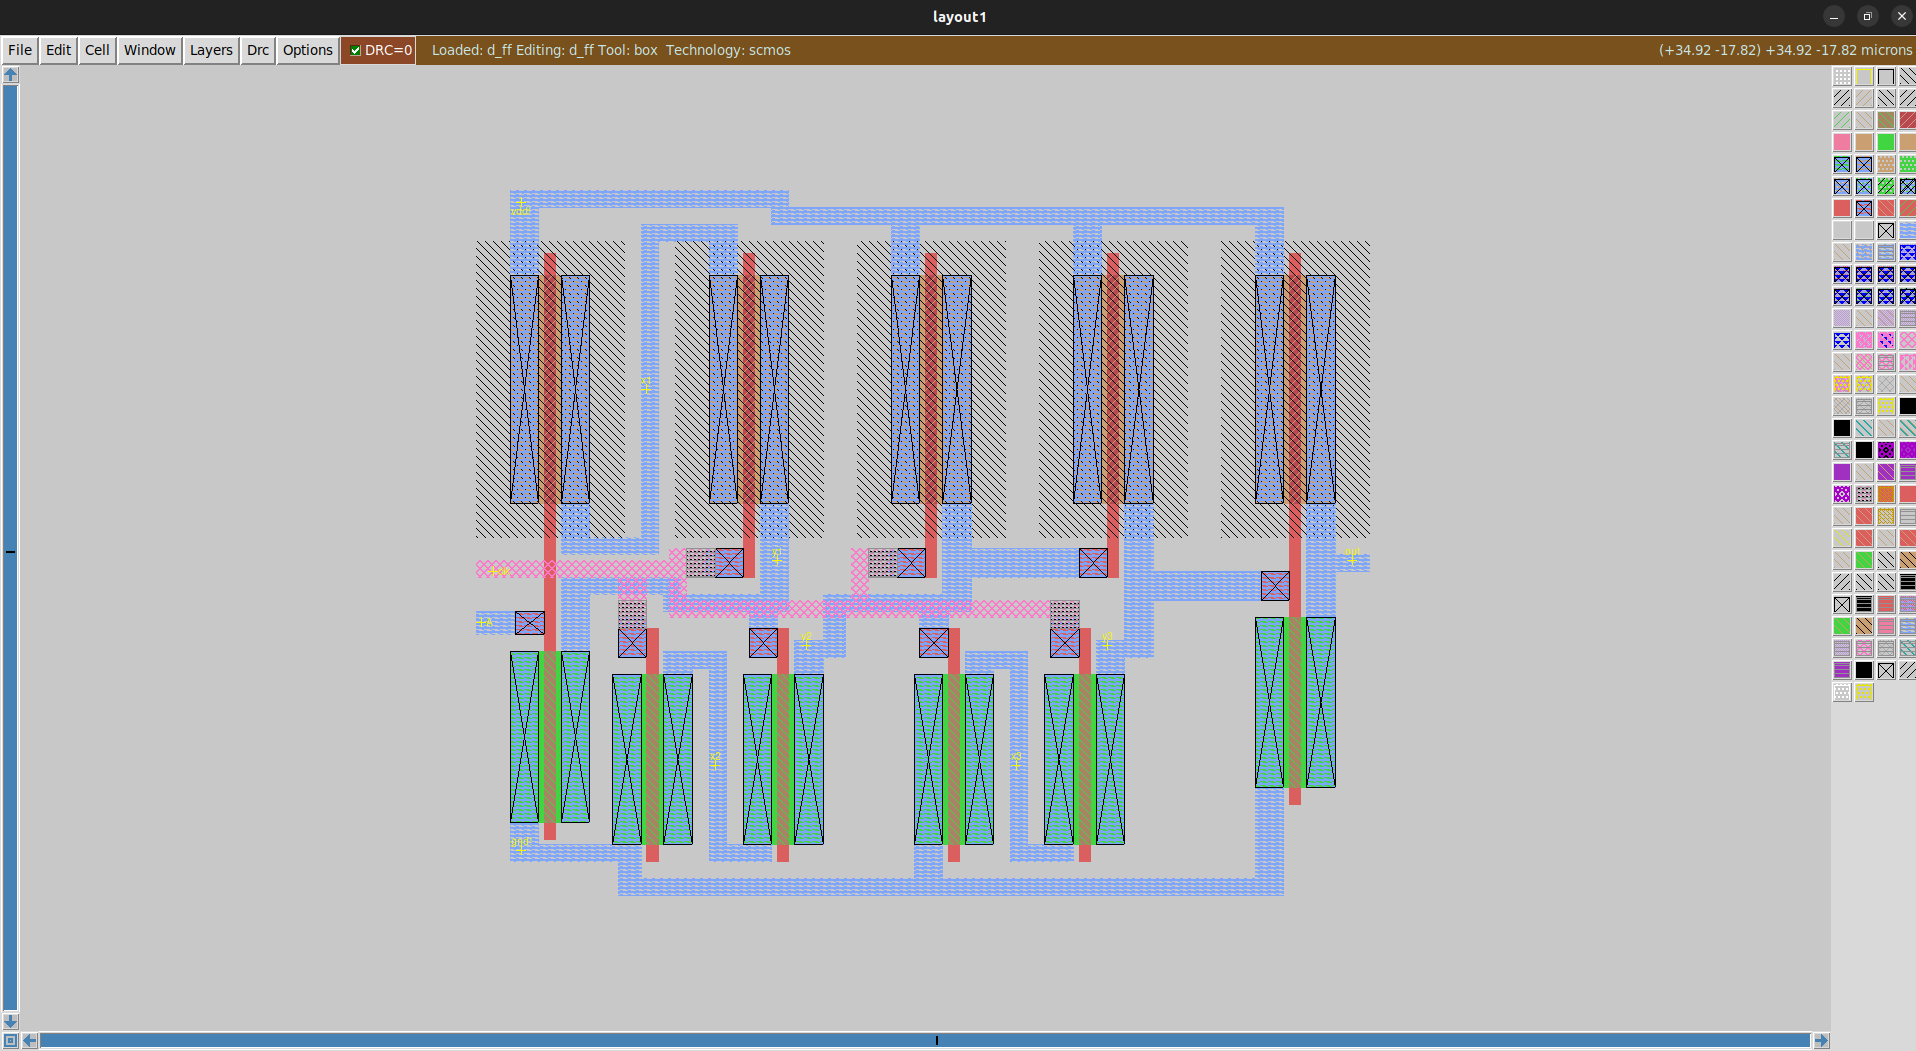
\includegraphics[width=0.45\textwidth]{/home/sudhujoshi/Desktop/Sem_3/VLSI/VLSI_Project/ReportDump/layout_ss/layout_d_ff.png}
    \caption{MAGIC Layout, D\_FF} 
\end{figure}

\begin{figure}[H] 
    \centering
    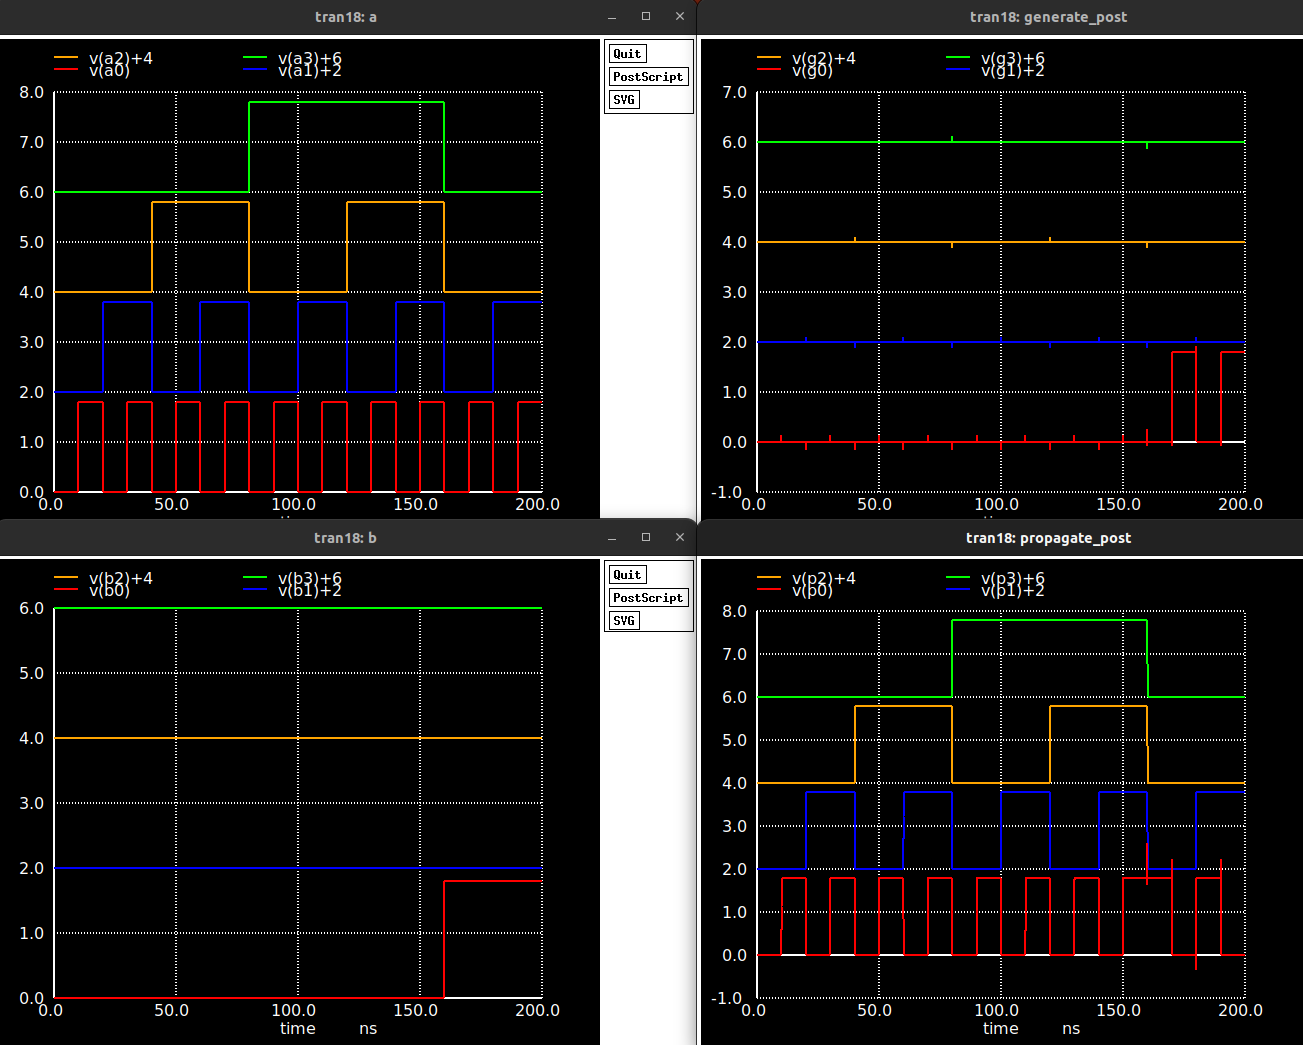
\includegraphics[width=0.45\textwidth]{/home/sudhujoshi/Desktop/Sem_3/VLSI/VLSI_Project/ReportDump/layout_ss/layout_propgen_sum.png}
    \caption{PropGen \& Sum Block Analysis} 
\end{figure}


% \begin{figure}[H] 
%     \centering
%     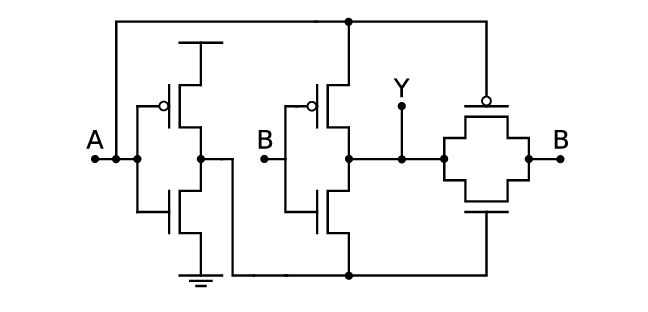
\includegraphics[width=0.4\textwidth]{/home/sudhujoshi/Desktop/Sem_3/VLSI/VLSI_Project/ReportDump/circuit_diagrams/exor_transmission.png}
%     \caption{MAGIC Layout, } 
% \end{figure}


\section{Block Integration}
\textbf{Note:} The modular implementation is in the \textbf{netlist-CLA} folder. 
All Logic Gates are referenced in a subcircuit file for readibility.
Netlists, Plots, etc are all available in respective folders.
\begin{figure}[H] 
    \centering
    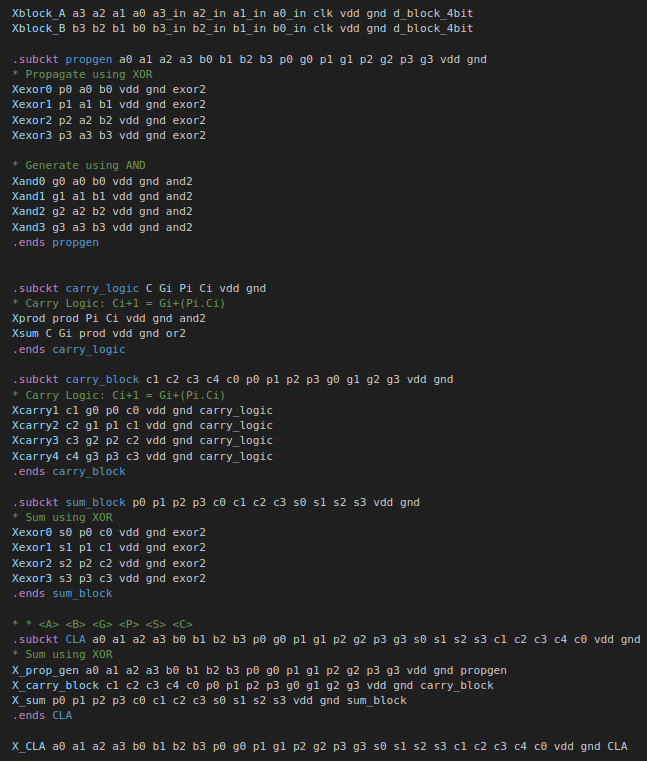
\includegraphics[width=0.35\textwidth]{/home/sudhujoshi/Desktop/Sem_3/VLSI/VLSI_Project/ReportDump/netlist_ss/integrated_netlist.png}
    \caption{Modular Netlist} 
\end{figure}
\begin{figure}[H] 
    \centering
    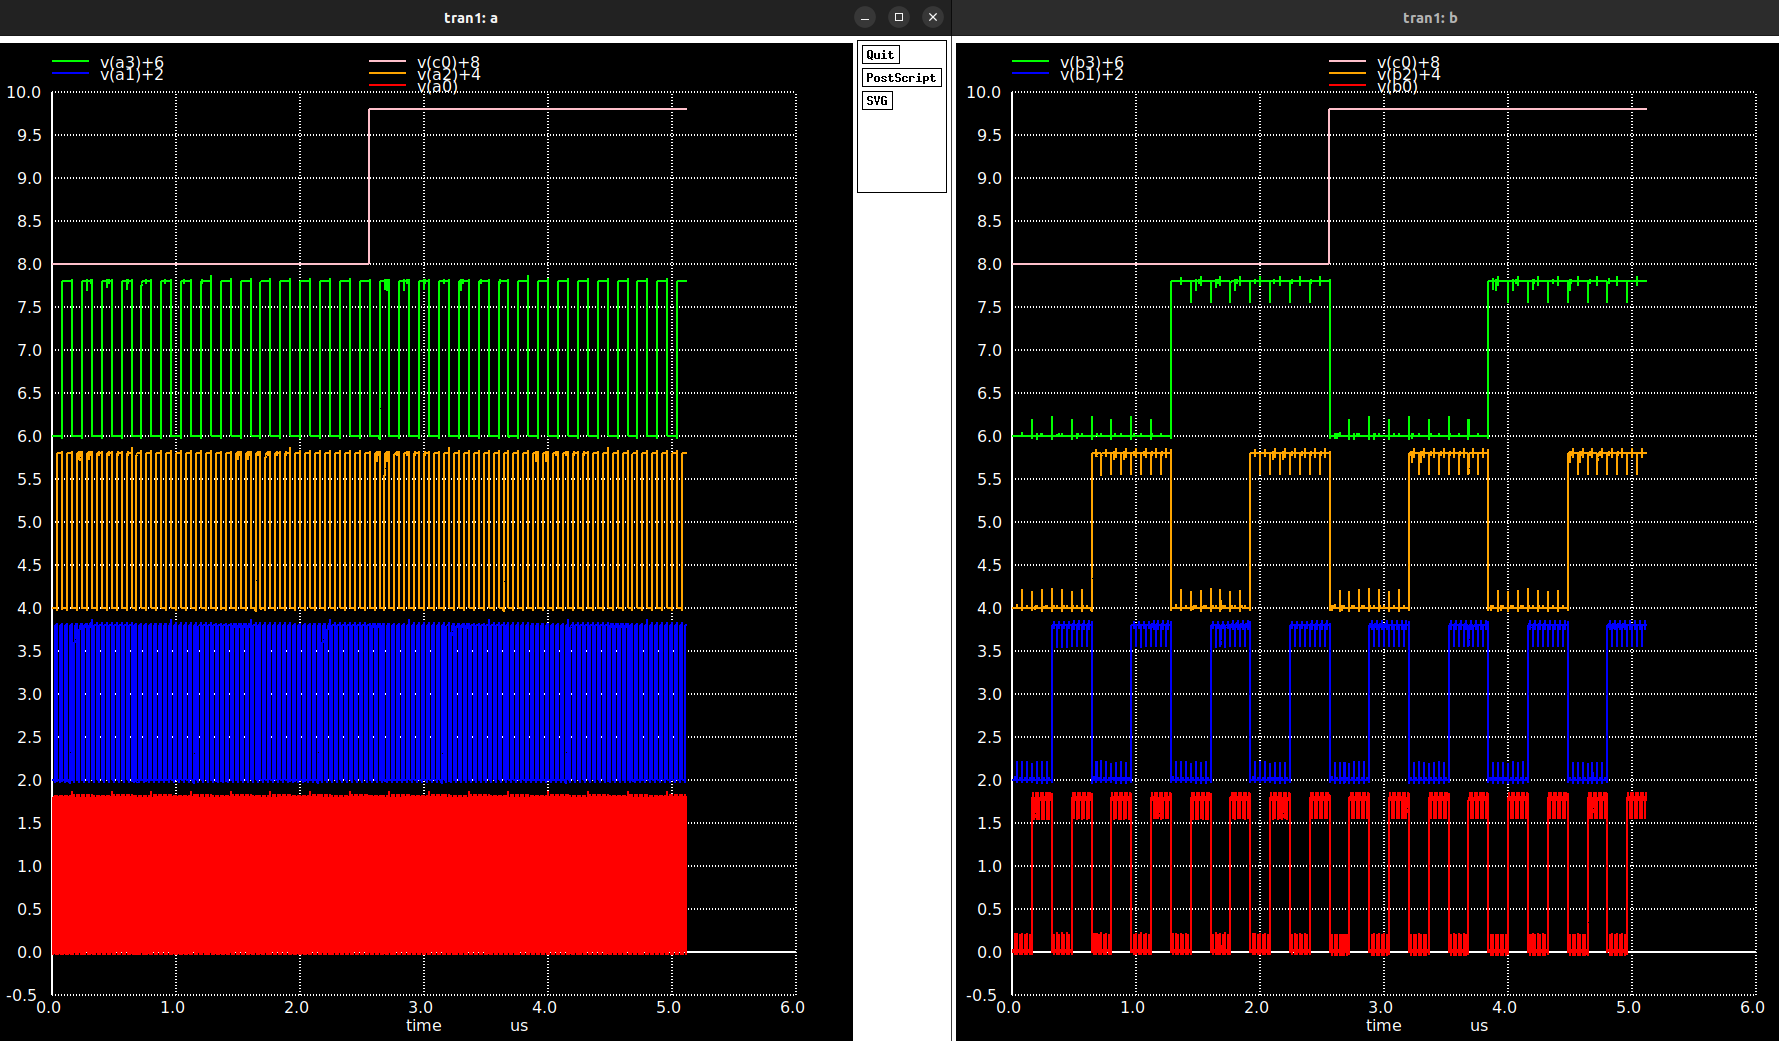
\includegraphics[width=0.35\textwidth]{/home/sudhujoshi/Desktop/Sem_3/VLSI/VLSI_Project/ReportDump/netlist_ss/inputs.png}
    \caption{A, B} 
\end{figure}
\begin{figure}[H] 
    \centering
    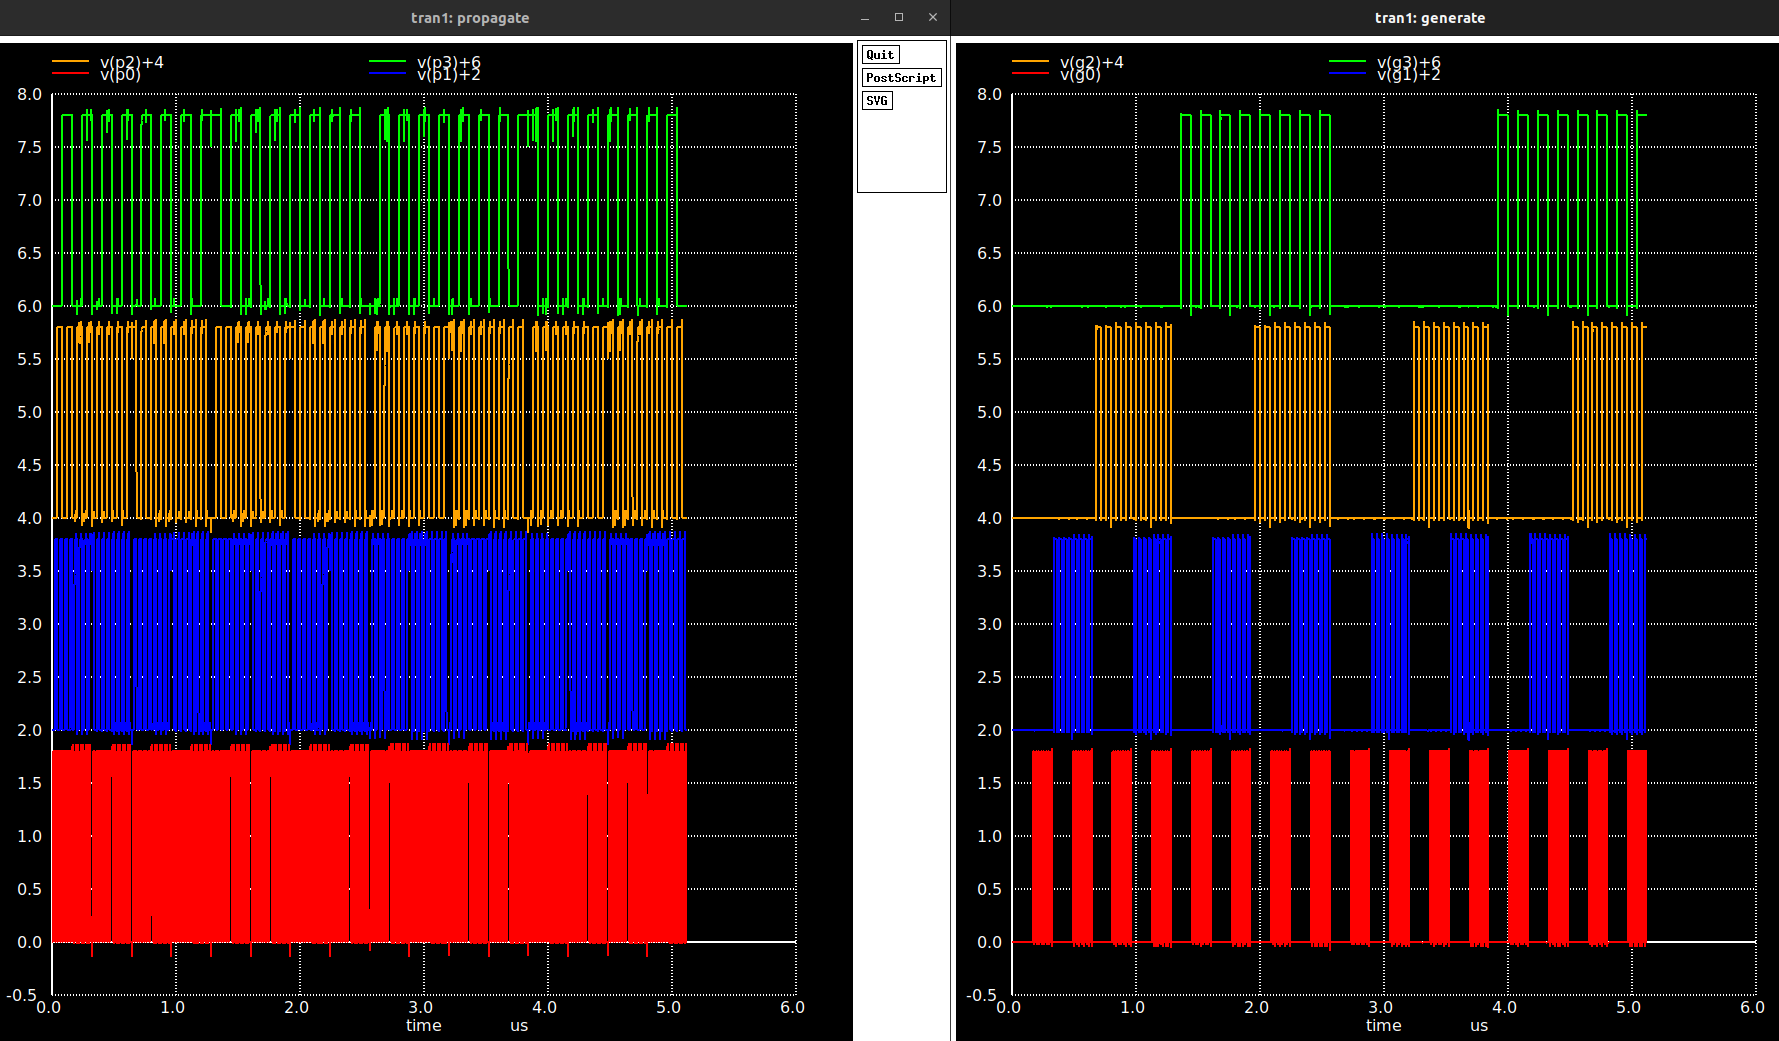
\includegraphics[width=0.35\textwidth]{/home/sudhujoshi/Desktop/Sem_3/VLSI/VLSI_Project/ReportDump/netlist_ss/propgen.png}
    \caption{Propagate, Generate} 
\end{figure}
\begin{figure}[H] 
    \centering
    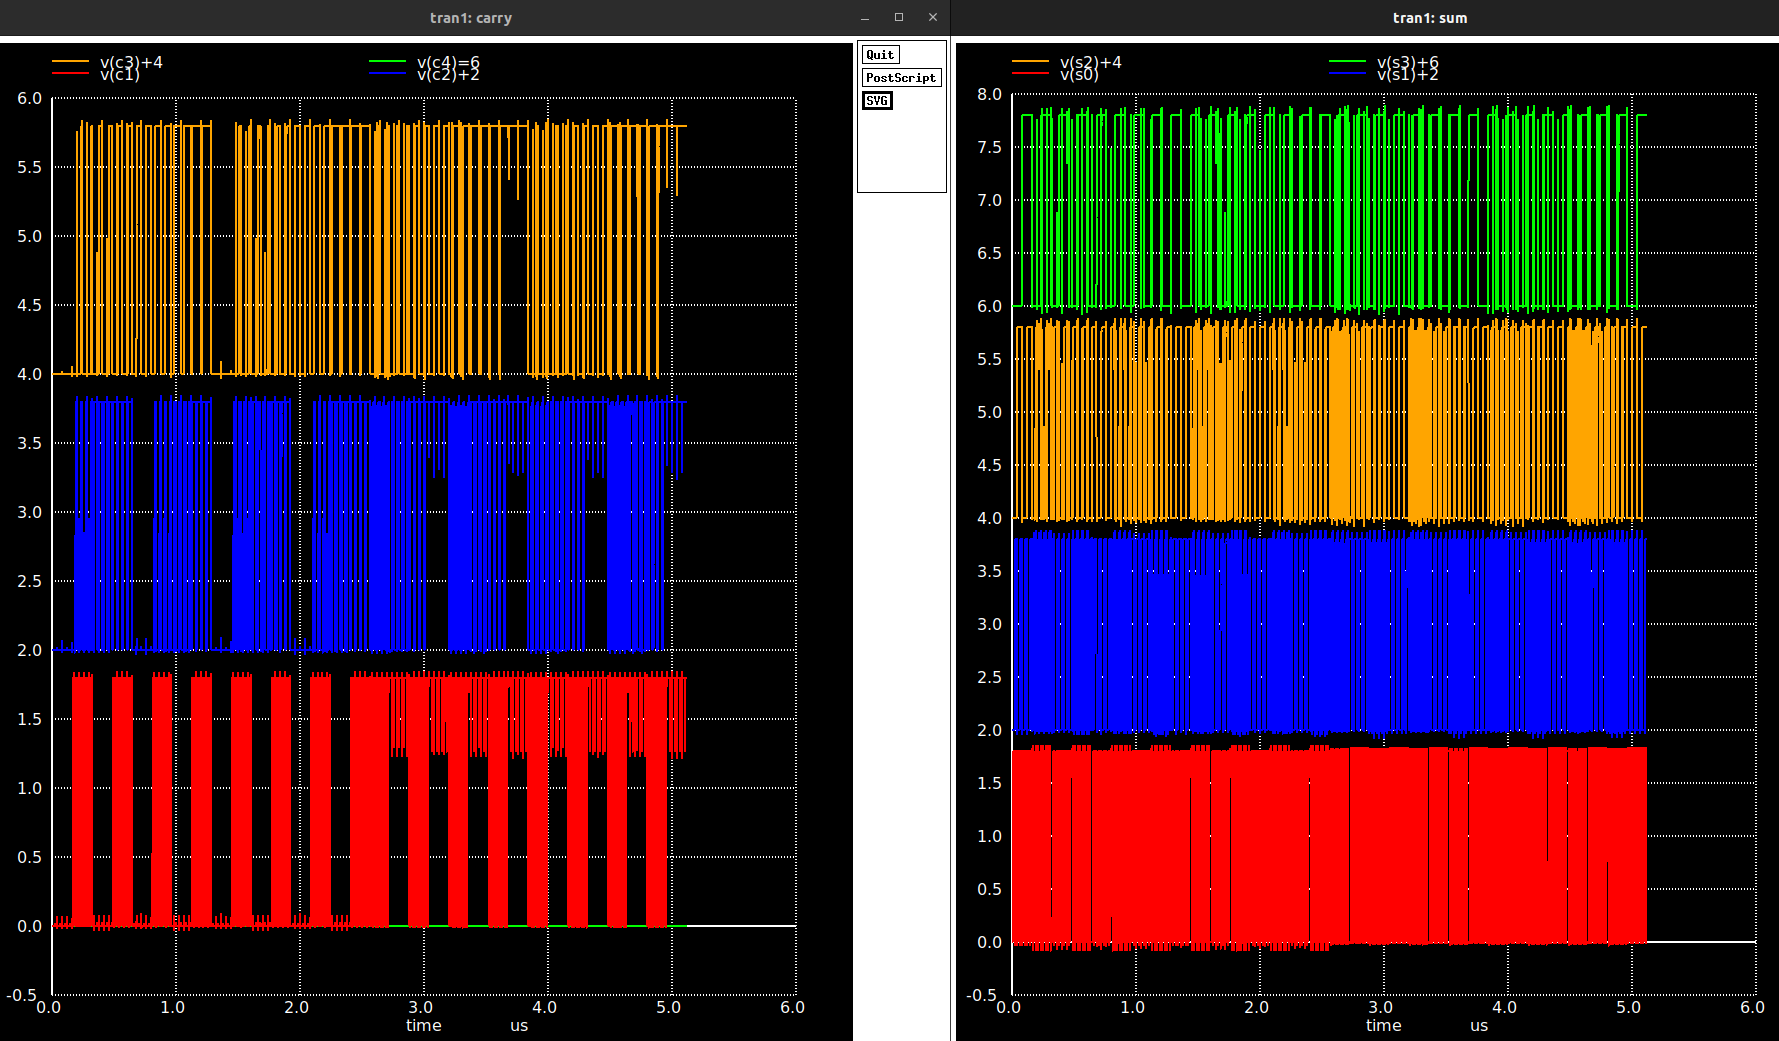
\includegraphics[width=0.35\textwidth]{/home/sudhujoshi/Desktop/Sem_3/VLSI/VLSI_Project/ReportDump/netlist_ss/carrysum.png}
    \caption{Carry, Sum} 
\end{figure}

Worst case delay will naturally occur for \( C_{out}\), due to largest gates and heaviest
logic function leading into this output.
\[
d_{max} \approx 0.26282\cdot10^{-9}s
\]

\[
f_{max} \approx \frac{1}{0.26282} \cdot 10^{9}
\]
\[
\therefore f_{max} \approx 3.8\cdot 10^{9} Hz
\]


\section{Floor Plan}
Assuming that the floor plan refers to the comprehensive final layout \& that 'pitches' 
refer to dimensions of our adder, the following design is implemented with corresponding 
labels for extraction to \textbf{spice netlist}.
\begin{figure}[H] 
    \centering
    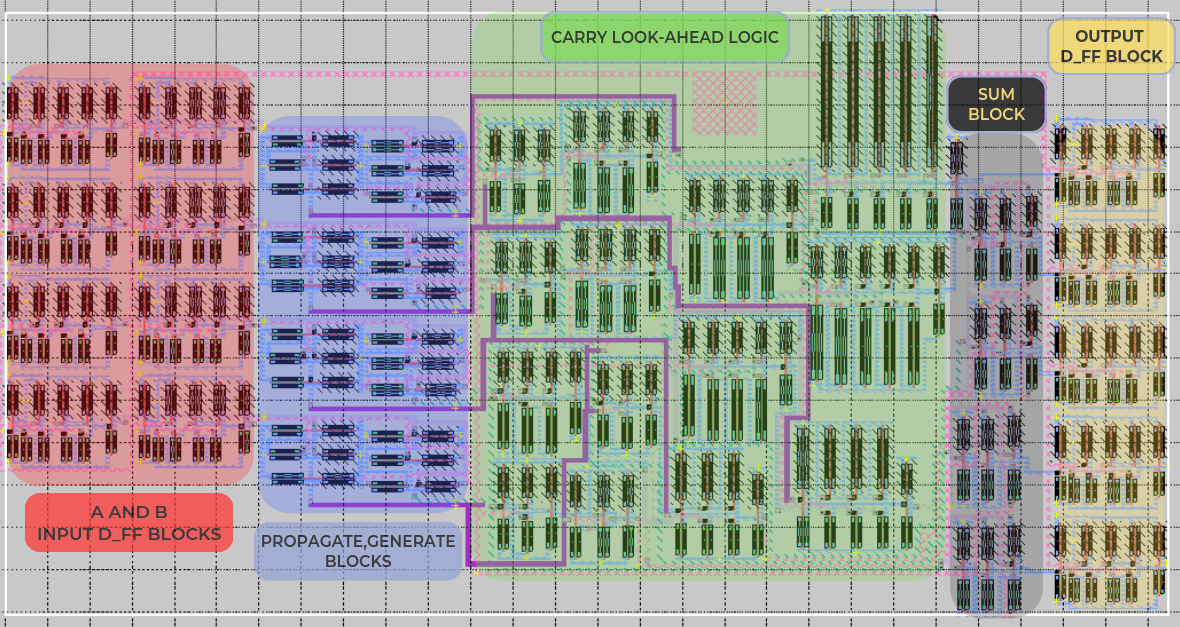
\includegraphics[width=0.45\textwidth]{/home/sudhujoshi/Desktop/Sem_3/VLSI/VLSI_Project/ReportDump/layout_ss/highlight_cla_layout.png}
    \caption{Highlighted Layout} 
\end{figure}

Dimensions occupied by the entire CLA block are:
\[
Area \approx 140\cdot72\;microns
\]

\section{Complete Circuit Post-Layout Simulation}
Final Layout is as follows:
\begin{figure}[H] 
    \centering
    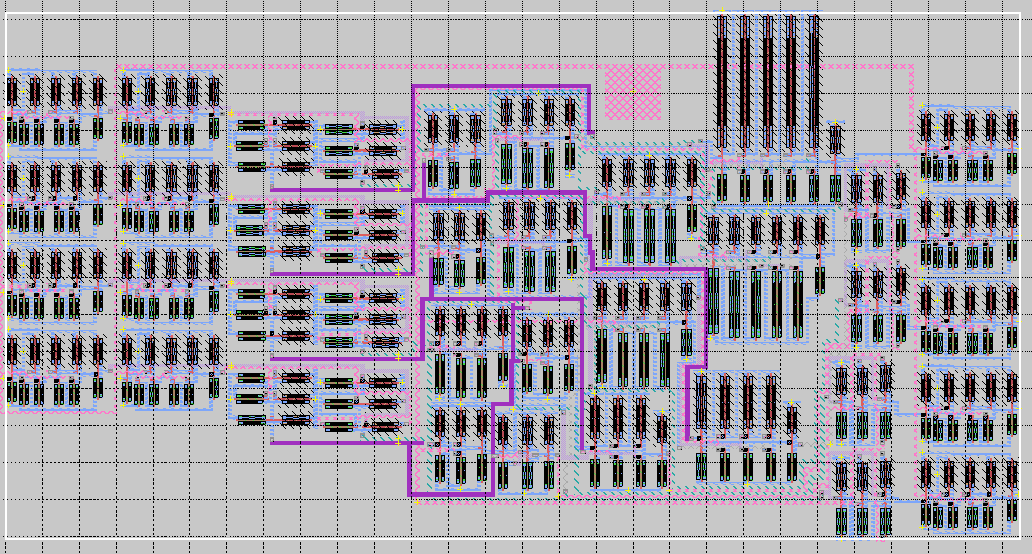
\includegraphics[width=0.45\textwidth]{/home/sudhujoshi/Desktop/Sem_3/VLSI/VLSI_Project/ReportDump/layout_ss/cla_layout.png}
    \caption{Final CLA Layout} 
\end{figure}
Comparing our schematic netlists with the post-layout extracted netlists:

\begin{figure}[H] 
    \centering
    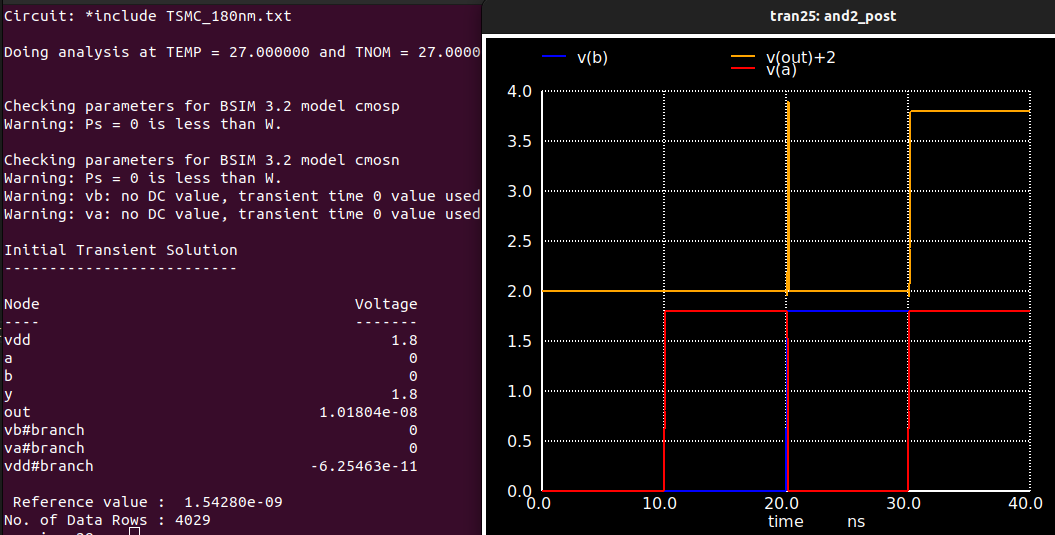
\includegraphics[width=0.4\textwidth]{/home/sudhujoshi/Desktop/Sem_3/VLSI/VLSI_Project/ReportDump/layout_ss/and2_post.png}
    \caption{AND2, Post Layout} 
\end{figure}
\begin{figure}[H] 
    \centering
    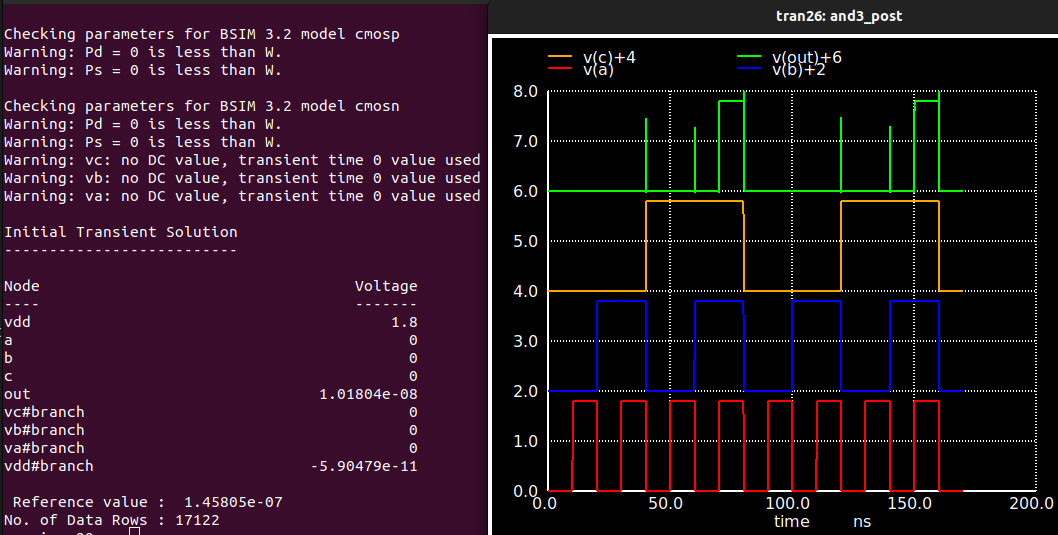
\includegraphics[width=0.4\textwidth]{/home/sudhujoshi/Desktop/Sem_3/VLSI/VLSI_Project/ReportDump/layout_ss/and3_post.png}
    \caption{AND3, Post Layout} 
\end{figure}
\begin{figure}[H] 
    \centering
    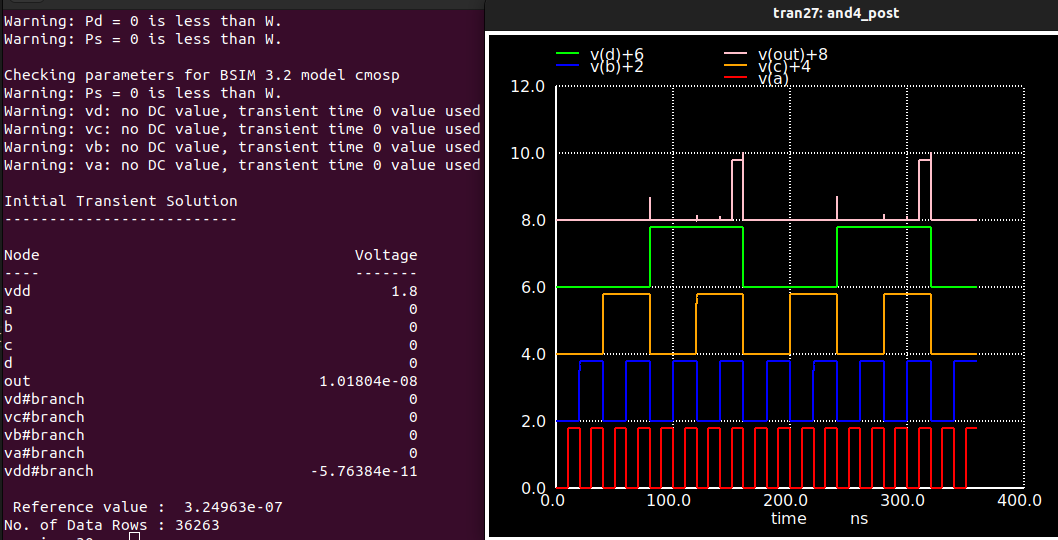
\includegraphics[width=0.4\textwidth]{/home/sudhujoshi/Desktop/Sem_3/VLSI/VLSI_Project/ReportDump/layout_ss/and4_post.png}
    \caption{AND4, Post Layout} 
\end{figure}
\begin{figure}[H] 
    \centering
    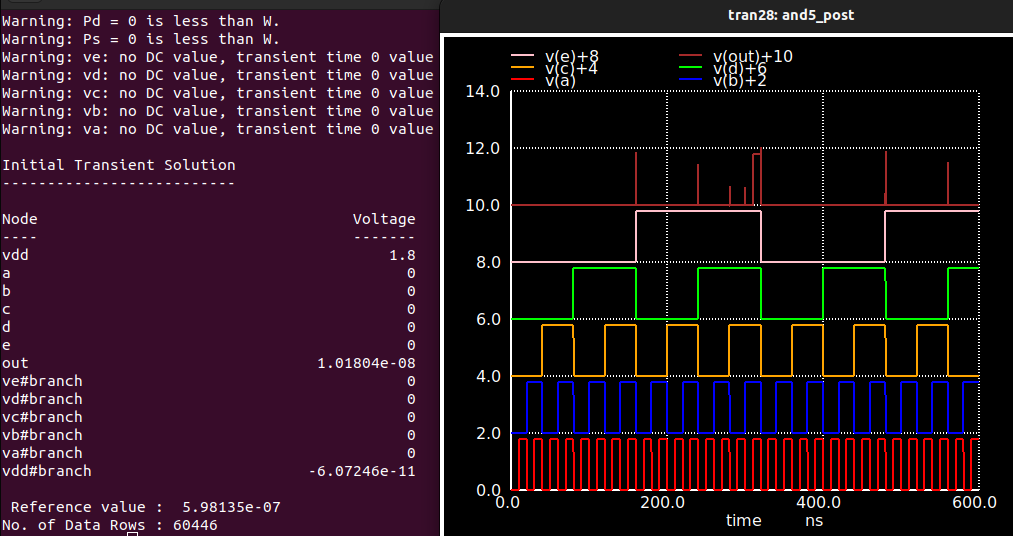
\includegraphics[width=0.4\textwidth]{/home/sudhujoshi/Desktop/Sem_3/VLSI/VLSI_Project/ReportDump/layout_ss/and5_post.png}
    \caption{AND5, Post Layout} 
\end{figure}



\begin{figure}[H] 
    \centering
    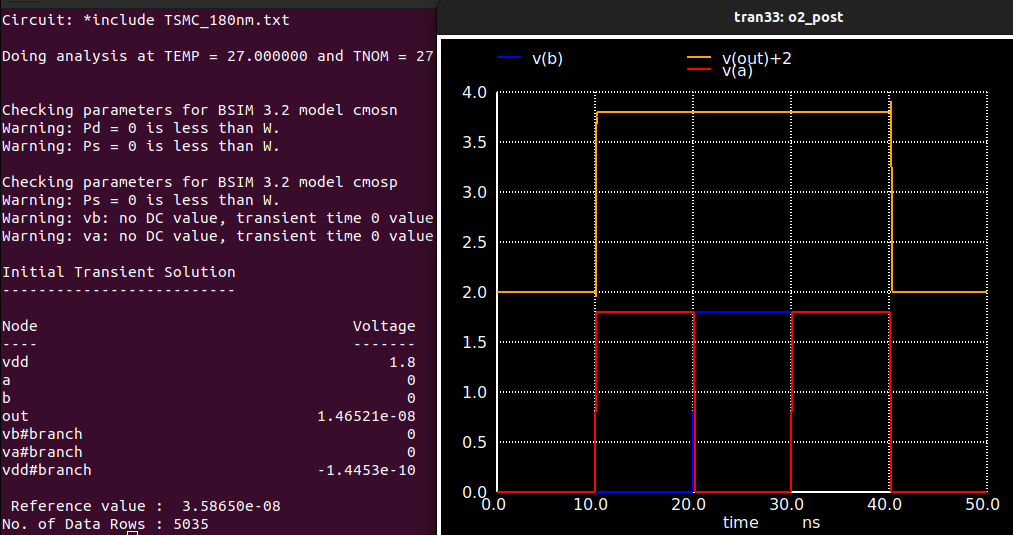
\includegraphics[width=0.4\textwidth]{/home/sudhujoshi/Desktop/Sem_3/VLSI/VLSI_Project/ReportDump/layout_ss/or2_post.png}
    \caption{OR2, Post Layout} 
\end{figure}
\begin{figure}[H] 
    \centering
    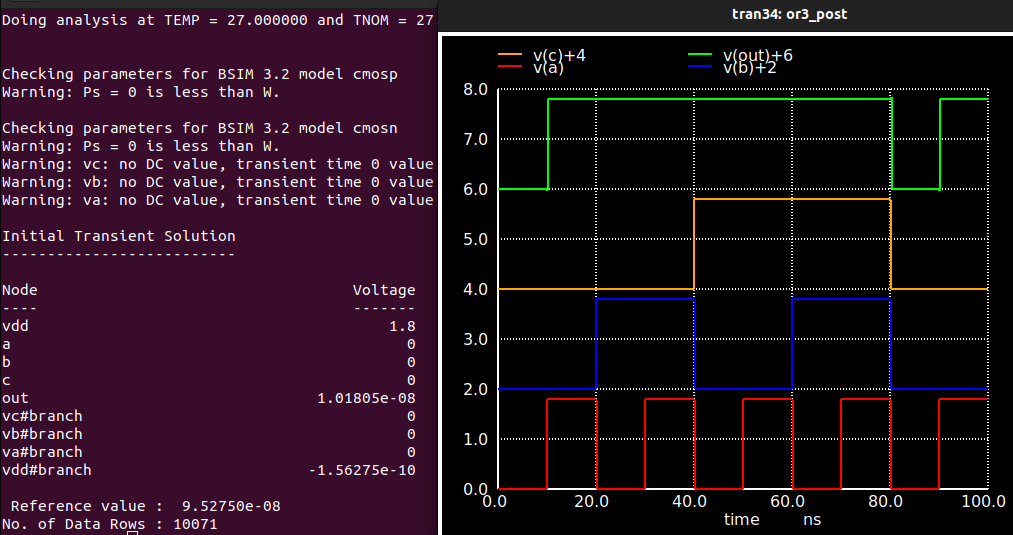
\includegraphics[width=0.4\textwidth]{/home/sudhujoshi/Desktop/Sem_3/VLSI/VLSI_Project/ReportDump/layout_ss/or3_post.png}
    \caption{OR3, Post Layout} 
\end{figure}
\begin{figure}[H] 
    \centering
    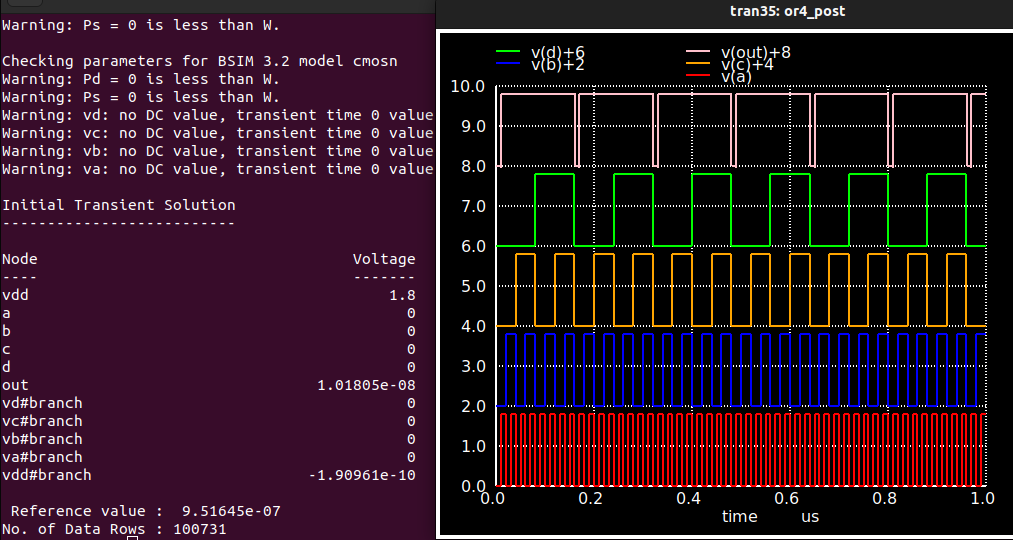
\includegraphics[width=0.4\textwidth]{/home/sudhujoshi/Desktop/Sem_3/VLSI/VLSI_Project/ReportDump/layout_ss/or4_post.png}
    \caption{OR4, Post Layout} 
\end{figure}
\begin{figure}[H] 
    \centering
    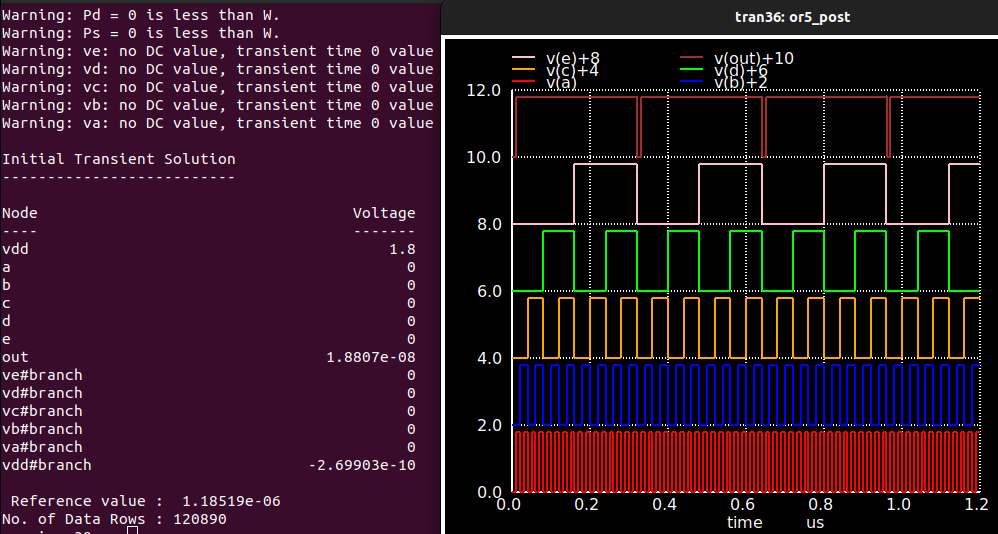
\includegraphics[width=0.4\textwidth]{/home/sudhujoshi/Desktop/Sem_3/VLSI/VLSI_Project/ReportDump/layout_ss/or5_post.png}
    \caption{OR5, Post Layout} 
\end{figure}


\begin{figure}[H] 
    \centering
    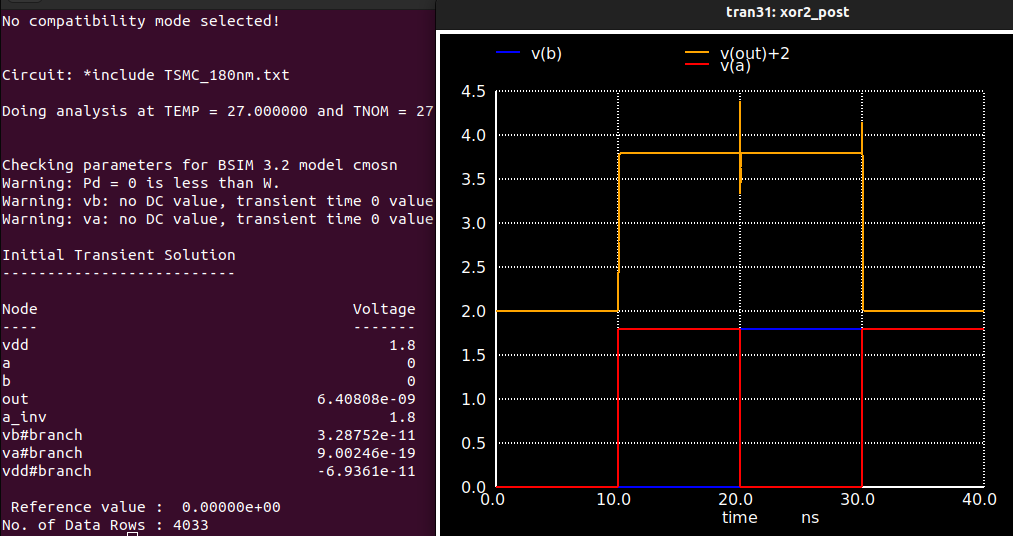
\includegraphics[width=0.35\textwidth]{/home/sudhujoshi/Desktop/Sem_3/VLSI/VLSI_Project/ReportDump/layout_ss/exor2_post.png}
    \caption{XOR2, Post Layout} 
\end{figure}
\begin{figure}[H] 
    \centering
    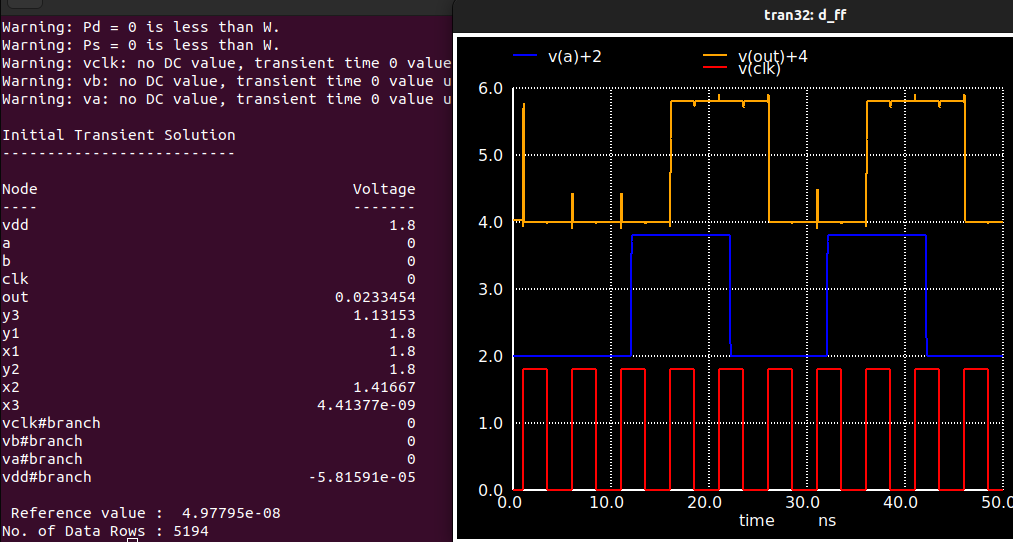
\includegraphics[width=0.35\textwidth]{/home/sudhujoshi/Desktop/Sem_3/VLSI/VLSI_Project/ReportDump/layout_ss/d_ff_post.png}
    \caption{D\_FF, Post Layout} 
\end{figure}

\begin{figure}[H] 
    \centering
    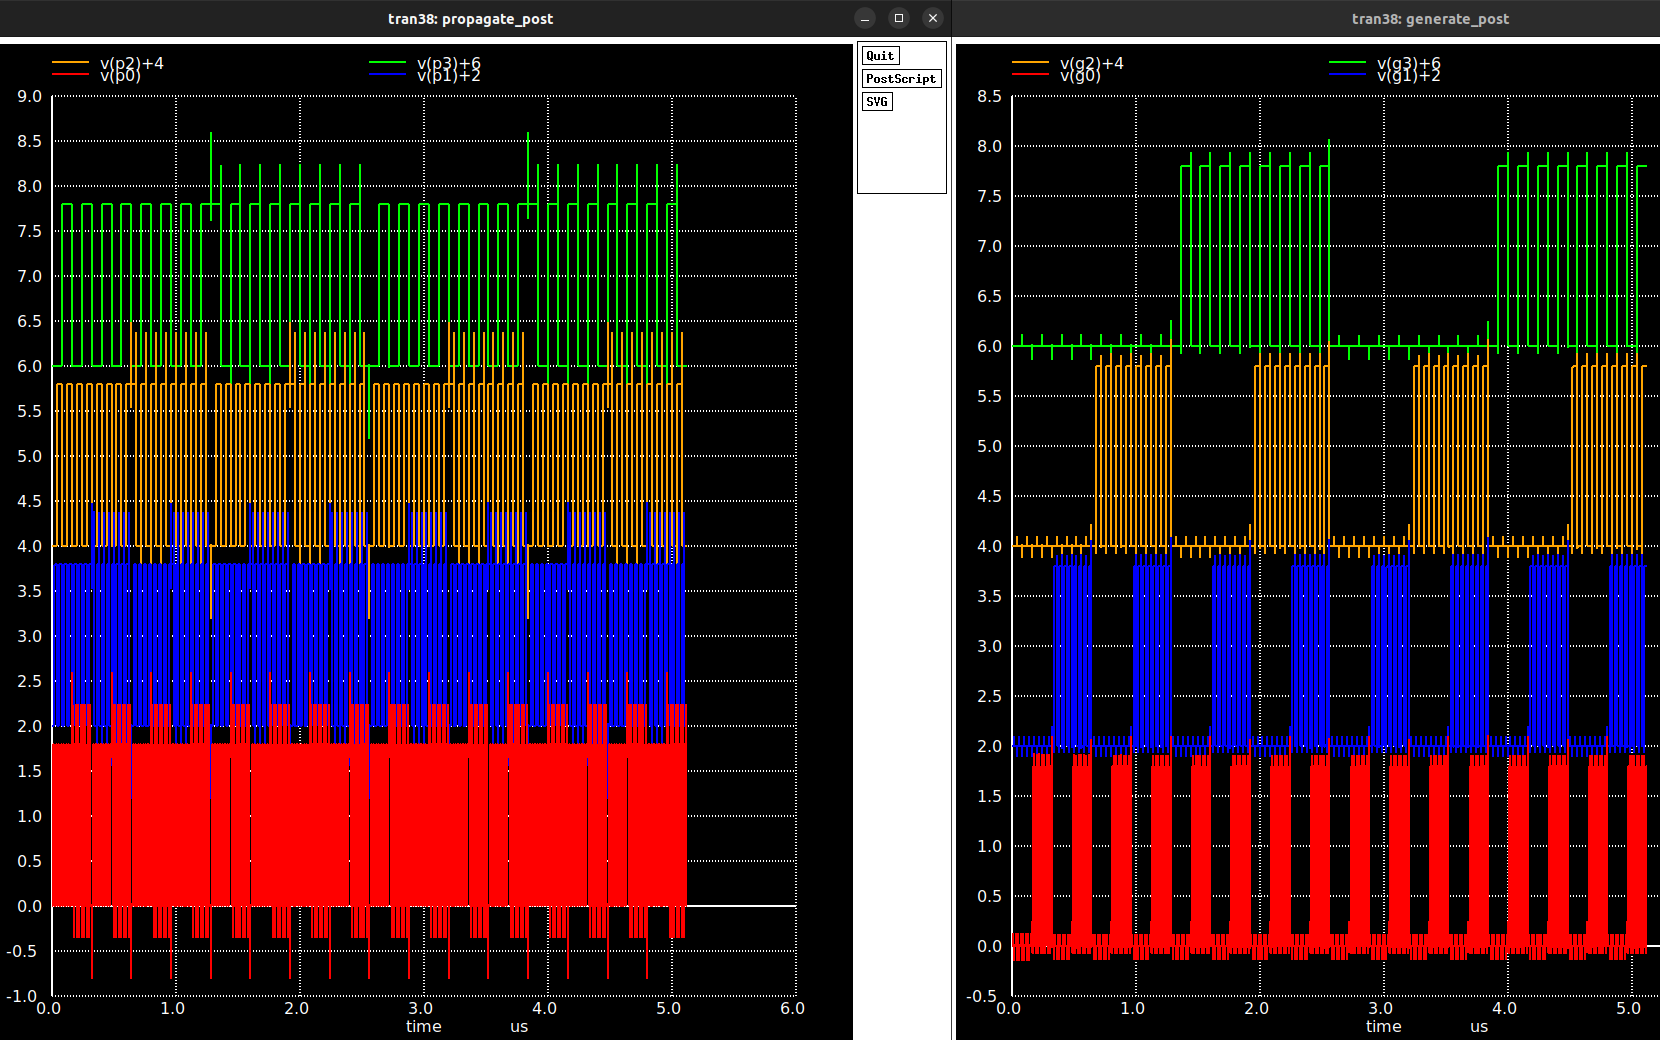
\includegraphics[width=0.35\textwidth]{/home/sudhujoshi/Desktop/Sem_3/VLSI/VLSI_Project/ReportDump/layout_ss/propgen_post.png}
    \caption{Propagate + Generate, Post Layout} 
\end{figure}
\begin{figure}[H] 
    \centering
    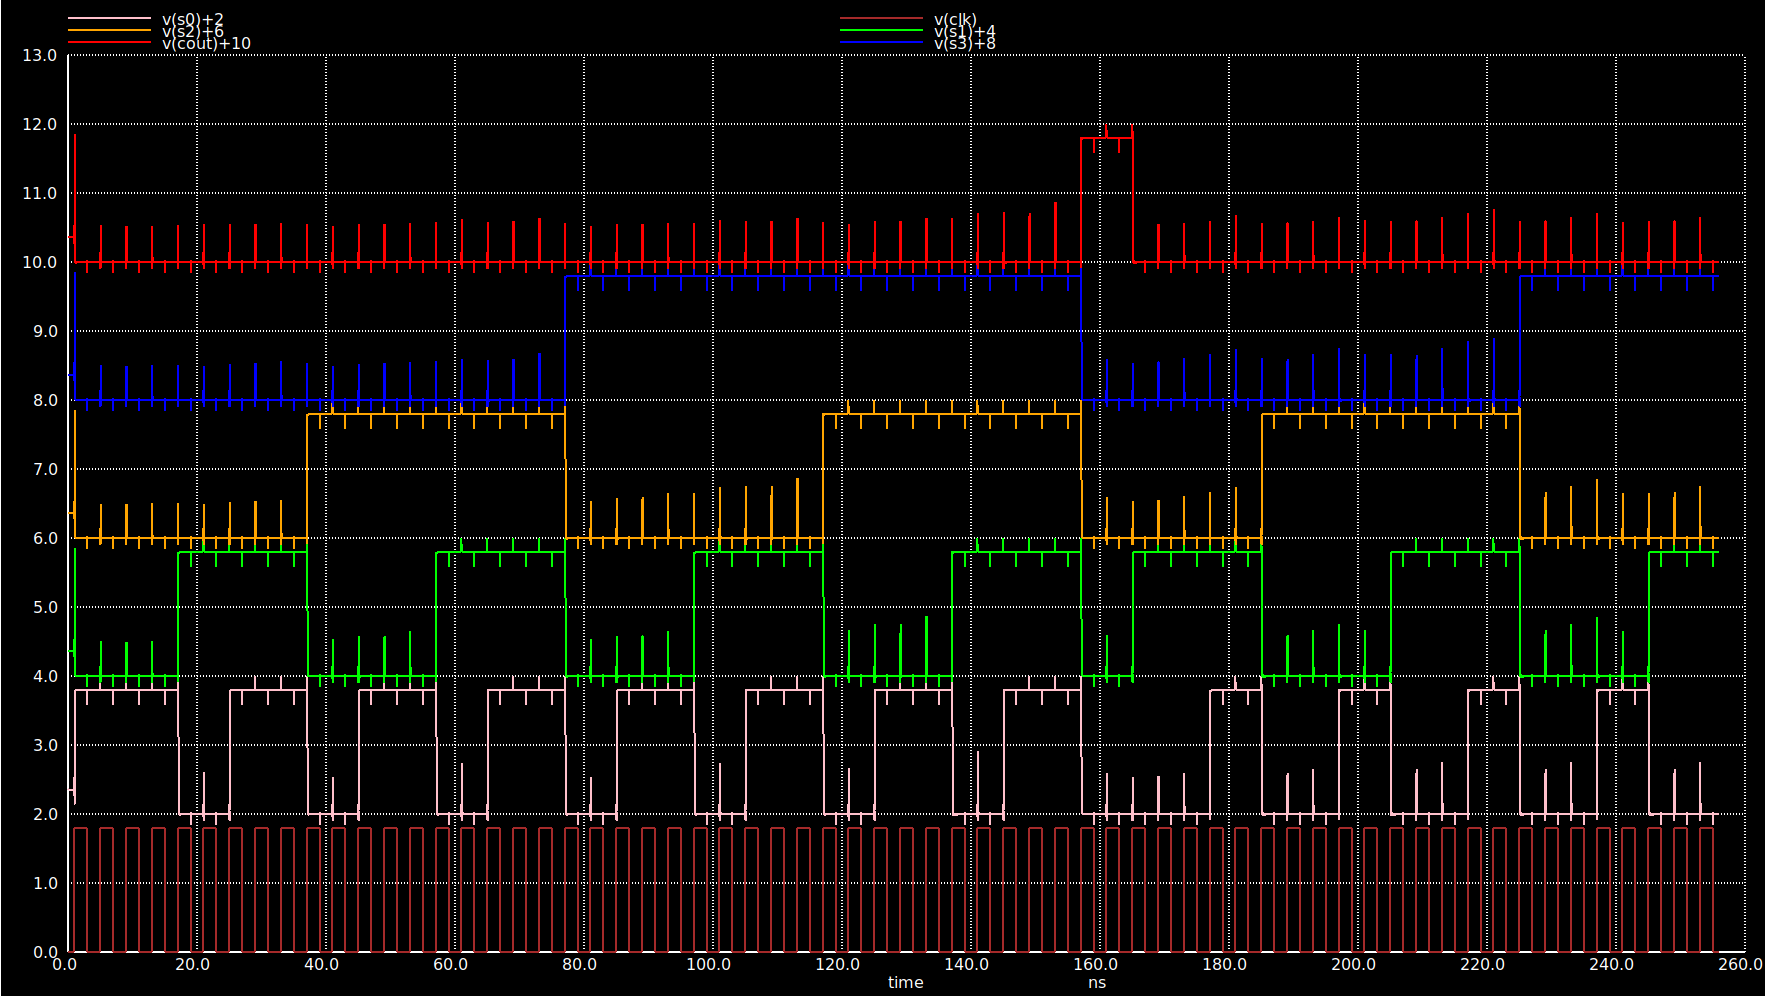
\includegraphics[width=0.35\textwidth]{/home/sudhujoshi/Desktop/Sem_3/VLSI/VLSI_Project/ReportDump/layout_ss/sum_post.png}
    \caption{Sum, Post Layout, Low Sweep} 
\end{figure}


\begin{table}[H]
    \centering
    \begin{tabular}{|c|c|c|}
    \hline
    \textbf{Parameter}             & \textbf{Schematic Simulation} & \textbf{Post-Layout Simulation} \\ \hline
    \textbf{Rise Time}             & $0.1342\cdot10^{-9}ns$       & $0.1567\cdot10^{-9}ns$        \\ \hline
    \textbf{Fall Time}             & $0.1041\cdot10^{-9}ns$       & $0.1338\cdot10^{-9}ns$        \\ \hline
    \textbf{Propagation Delay}     & $0.2903\cdot10^{-9}ns$       & $0.3092\cdot10^{-9}ns$         \\ \hline
    \textbf{Propagate Signal Delay}& $0.2706\cdot10^{-9}ns$       & $0.3105\cdot10^{-9}ns$         \\ \hline
    \textbf{Generate Signal Delay} & $0.2691\cdot10^{-9}ns$       & $0.2874\cdot10^{-9}ns$         \\ \hline
    \textbf{Sum Output Delay}      & $0.2952\cdot10^{-9}ns$       & $0.3109\cdot10^{-9}ns$         \\ \hline
    \textbf{Carry Output Delay}    & $0.2709\cdot10^{-9}ns$       & $0.3013\cdot10^{-9}ns$          \\ \hline
    \end{tabular}
    \caption{Schematic \& Post-Layout Comparison}
    \label{tab:schematic_vs_postlayout, approximate}
\end{table}

% % \[
% % Fall Time = $0.13388\cdot10^{-9}\;Rise Time = $0.15677\cdot10^{-9}
% % \]
% \\
% Defining \textbf{Clock-to-Q} delay as the time taken for the input change to propagate from the rising edge of the clock to the output \( Q \), we obtain the result through plot observation: 
% \[
% t_{CtQ} \approx 0.1731\cdot10^{-9}s
% \]
% \[
% t_{prop} \approx 0.10438\cdot10^{-9}s
% \]
    

    
\section{Delay, Clock Frequency Contraints}
Worst case delay will naturally occur for \( C_{out}\) again.
\[
d_{max} \approx 0.3047\cdot10^{-9}s
\]

\[
f_{max} \approx \frac{1}{0.3047} \cdot 10^{9}
\]
\[
\therefore f_{max} \approx 3.2819\cdot 10^{9} Hz
\]

\section{Verilog HDL}
\begin{figure}[H] 
    \centering
    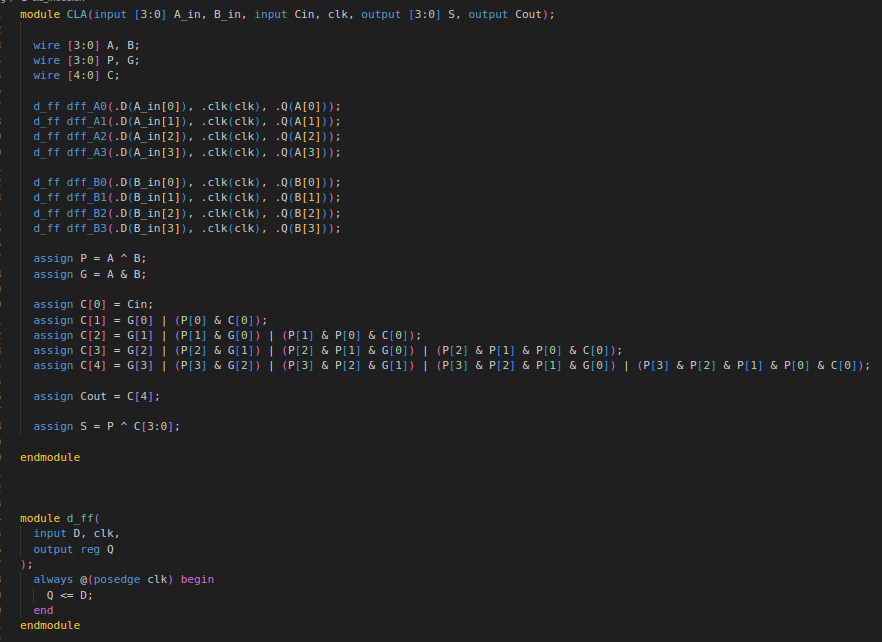
\includegraphics[width=0.35\textwidth]{/home/sudhujoshi/Desktop/Sem_3/VLSI/VLSI_Project/ReportDump/verilog_ss/module.png}
    \caption{Verilog Modules, CLA \& D Flip-Flop} 
\end{figure}
\begin{figure}[H] 
    \centering
    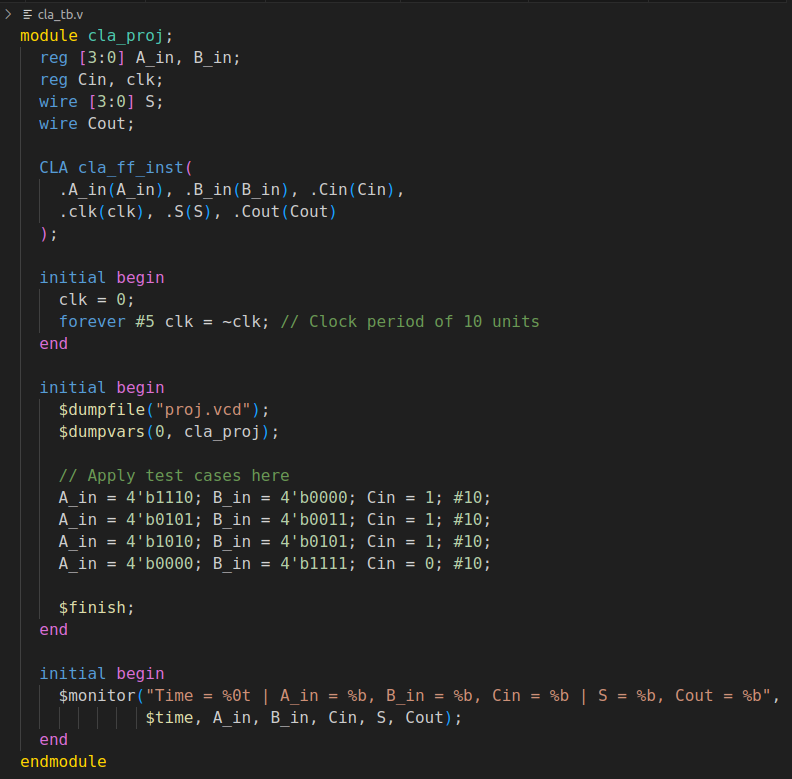
\includegraphics[width=0.35\textwidth]{/home/sudhujoshi/Desktop/Sem_3/VLSI/VLSI_Project/ReportDump/verilog_ss/testbench.png}
    \caption{Testbench, Verilog HDL} 
\end{figure}
\begin{figure}[H] 
    \centering
    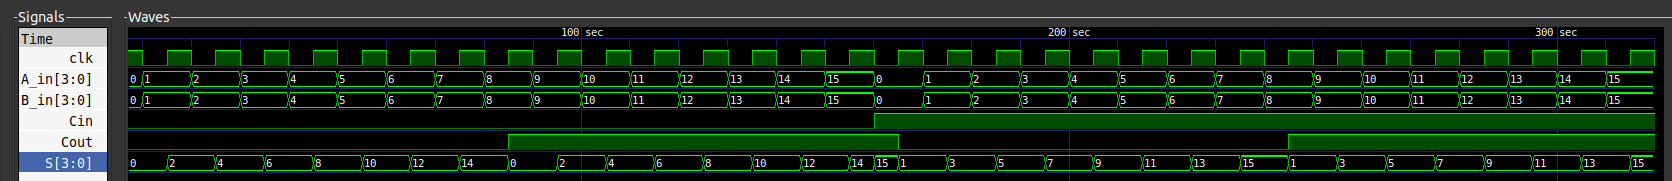
\includegraphics[width=0.4\textwidth]{/home/sudhujoshi/Desktop/Sem_3/VLSI/VLSI_Project/ReportDump/verilog_ss/gtkwave.png}
    \caption{Waveforms, GTKWave} 
\end{figure}
\begin{figure}[H] 
    \centering
    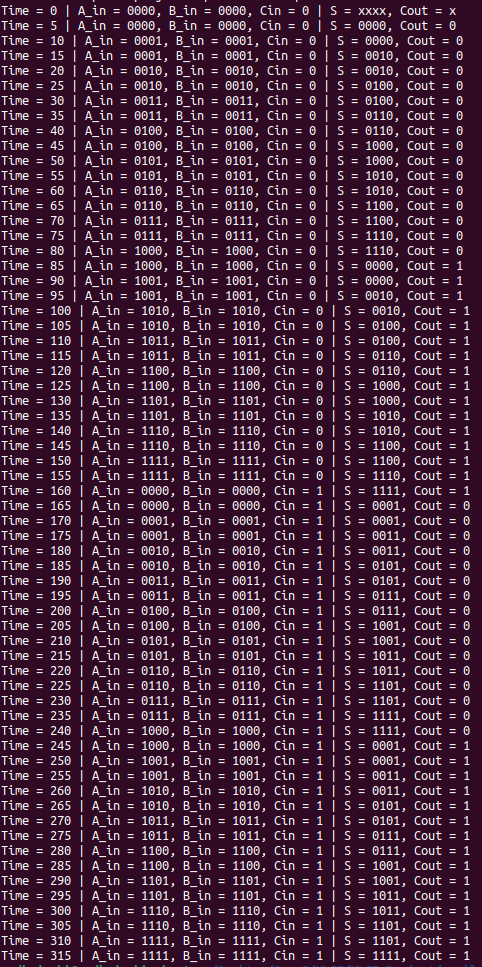
\includegraphics[width=0.25\textwidth]{/home/sudhujoshi/Desktop/Sem_3/VLSI/VLSI_Project/ReportDump/verilog_ss/verilog_res.png}
    \caption{Truth Table, Verilog} 
\end{figure}


\section{FPGA, Oscilloscope Implementation}
The following links contain brief video demonstrations of FPGA Implementation and 
Generations of Oscilloscope Waveforms using an Arduino UNO.

\href{https://drive.google.com/drive/folders/15TUTqYzhG3WnAiuiNixyvRwzI8kM6A_v?usp=drive_link}
{FPGA \& Oscilloscope Demo, Google Drive}

\begin{figure}[H] 
    \centering
    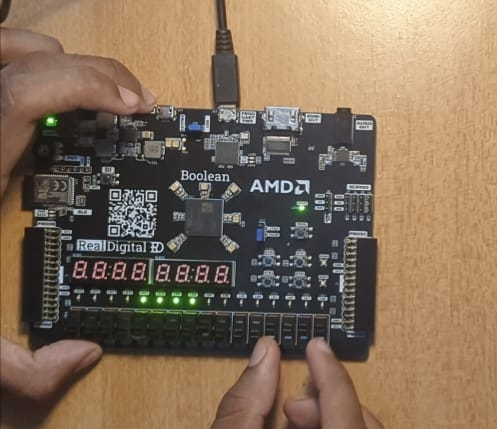
\includegraphics[width=0.3\textwidth]{/home/sudhujoshi/Desktop/Sem_3/VLSI/VLSI_Project/ReportDump/verilog_ss/board.png}
    \caption{Vivado Test, AMD Boolean Board} 
\end{figure}
\begin{figure}[H] 
    \centering
    \includegraphics[width=0.3\textwidth]{/home/sudhujoshi/Desktop/Sem_3/VLSI/VLSI_Project/ReportDump/verilog_ss/oscilloscope.png}
    \caption{Waveforms, GTKWave} 
\end{figure}

\section*{Acknowledgment}
I sincerely thank Professor Abhishek Shrivastava and the TAs for their invaluable 
guidance and support throughout this project, as their assistance and constructive 
feedback greatly contributed to the successful completion of this work.

\section*{References}
1. International Journal of Recent Technology and Engineering (IJRTE),  
   ISSN: 2277-3878 (Online), Volume-8, Issue-1, May 2019.  
   \href{https://www.ijrte.org/wp-content/uploads/papers/v8i1/A1382058119.pdf}{Available online} \\[0.5em]

2. Logic Design, Dinesh Sharma, Microelectronics Group, EE Department, IIT Bombay. \\[0.5em]

3. Carry-lookahead Adder, Wikipedia.  
\href{https://en.wikipedia.org/wiki/Carry-lookahead_adder}{Available online}




\end{document}